\chapter{Sistemas de ecuaciones lineales\\ Linear equation systems}\index{sistemas} \index[eng]{systems}
\chaptermark{Sistemas \textreferencemark\ Systems}
\epigraph{Después de cada guerra \\ alguien tiene que limpiar. \\ No se van a ordenar solas las cosas, \\ digo yo. (Maria Wisława Anna Szymborska)}

\begin{paracol}{2}

\section{Introducción}

Una ecuación lineal es aquella que establece una relación \emph{lineal} entre dos o más variables, por ejemplo,

\begin{equation*}
3x_1-2x_2=12
\end{equation*}

Se dice que es una relación lineal, porque las variables están relacionadas entre sí tan solo mediante sumas y productos por coeficientes constantes. En particular, el ejemplo anterior puede representarse geométricamente mediante una línea recta.

El número de variables relacionadas en una ecuación lineal determina la dimensión de la ecuación. La del ejemplo anterior es una ecuación bidimensional, puesto que hay dos variables. El número puede ser arbitrariamente grande en general,
\begin{equation*}
a_1x_1+a_2x_2+\cdots +a_nx_n=b
\end{equation*} 
será una ecuación n-dimensional.

\switchcolumn    

\section{Introduction}

A linear equation is an equation that establishes a \emph{linear} relationship between two or more variables, for example,

\begin{equation}
3x_1-2x_2=12
\end{equation}

It is said to be a linear relationship, because the variables are related to each other only through additions and products by constant coefficients. In particular, the above example can be represented geometrically by a straight line.

The number of related variables in a linear equation determines the dimension of the equation. The above example is a two-dimensional equation, since there are two variables. The number can be arbitrarily large in general,
\begin{equation*}
a_1x_1+a_2x_2+cdots +a_nx_n=b
\end{equation*} 
will be an n-dimensional equation.

\switchcolumn
Como ya hemos señalado más arriba, una ecuación bidimensional admite una línea recta como representación geométrica, una ecuación tridimensional admitirá un plano y para dimensiones mayores que tres cada ecuación representará un hiperplano de dimension n. Por supuesto, para dimensiones mayores que tres, no es posible obtener una representación gráfica de la ecuación.

Las ecuaciones lineales juegan un papel muy importante en la física y, en general en la ciencia y la tecnología. La razón es que constituyen la aproximación matemática más sencilla a la relación entre magnitudes físicas. Por ejemplo cuando decimos que la fuerza aplicada a un resorte y la elongación  que sufre están relacionadas por la ley de Hooke, $F=Kx$ estamos estableciendo una relación lineal entre las magnitudes fuerza y elongación. ¿Se cumple siempre dicha relación? Desde luego que no. Pero es razonablemente cierta para elongaciones pequeñas y, apoyados en ese sencillo modelo \emph{lineal} de la realidad, se puede aprender mucha física.

Un sistema de ecuaciones lineales está constituido por varias ecuaciones lineales, que expresan relaciones lineales distintas sobre las mismas variables. Por ejemplo,

\begin{align*}
a_{11}x_1+a_{12}x_2&=b_1\\
a_{21}x_1+a_{22}x_2&=b_2
\end{align*}

\switchcolumn
As we have already pointed out above, a two-dimensional equation admits a straight line as geometrical representation, a three-dimensional equation will admit a plane and for dimensions greater than three each equation will represent a hyperplane of dimension n. Of course, for dimensions greater than three, it is not possible to obtain a graphical representation of the equation.

Linear equations play a very important role in physics and, in general, in science and technology. The reason is that they are the simplest mathematical approximation of the relationship between physical quantities. For example, when we say that the force applied to a spring and the elongation it undergoes are related by Hooke's law, $F=Kx$, we are establishing a linear relationship between the quantities force and elongation. Does this relationship always hold true? Certainly not. But it is reasonably true for small elongations and, based on this simple \emph{linear} model of reality, a lot of physics can be learned.

A system of linear equations is made up of several linear equations, which express different linear relationships about the same variables. For example,

\begin{align*}
a_{11}x_1+a_{12}x_2&=b_1\\
a_{21}x_1+a_{22}x_2&=b_2
\end{align*}

\switchcolumn

Se llaman soluciones del sistema de ecuaciones a los valores de las variables que satisfacen simultáneamente a todas las ecuaciones que componen el sistema. Desde el punto de vista de la obtención de las soluciones a las variables se les suele denominar incógnitas, es decir valores no conocidos que deseamos obtener o calcular.

Un sistema de ecuaciones puede tener infinitas soluciones, puede tener una única solución o puede no tener solución. En lo que sigue, nos centraremos en sistemas de ecuaciones que tienen una única solución. 

Una primera condición para que un sistema de ecuaciones tengan una única solución es que el número de incógnitas presentes en el sistema coincida con el número de ecuaciones. 

\switchcolumn

The values of the variables that simultaneously satisfy all the equations that make up the system are called solutions of the system of equations. From the point of view of obtaining the solutions, the variables are usually called unknowns, i.e. unknown values that we wish to obtain or calculate.

A system of equations can have infinite solutions, it can have only one solution or it can have no solution. In what follows, we will focus on systems of equations that have only one solution. 

A first condition for a system of equations to have a unique solution is that the number of unknowns present in the system coincides with the number of equations. 

\switchcolumn

De modo general podemos decir que vamos a estudiar métodos numéricos para resolver con un computador sistemas de $n$ ecuaciones con $n$ incógnitas,

\begin{align*}
a_{11}&x_1+a_{12}x_2+\cdots +a_{1n}x_n=b_1\\
a_{21}&x_1+a_{22}x_2+\cdots +a_{2n}x_n=b_2\\
\cdots & \\
a_{n1}&x_1+a_{n2}x_2+\cdots +a_{nn}x_n=b_n
\end{align*}  

Una de las grandes ventajas de los sistemas de ecuaciones lineales es que puede expresarse en forma de producto matricial,

\switchcolumn

In general terms, we can say that we are going to study numerical methods to solve with a computer systems of $n$ equations with $n$ unknowns,

\begin{align*}
a_{11}&x_1+a_{12}x_2+\cdots +a_{1n}x_n=b_1\\
a_{21}&x_1+a_{22}x_2+\cdots +a_{2n}x_n=b_2\\
\cdots & \\
a_{n1}&x_1+a_{n2}x_2+\cdots +a_{nn}x_n=b_n
\end{align*}  

One of the great advantages of systems of linear equations is that they can be expressed in matrix product form,

\end{paracol}



\begin{equation*}
\left. \begin{aligned}
a_{11}&x_1+a_{12}x_2+\cdots +a_{1n}x_n=b_1\\
a_{21}&x_1+a_{22}x_2+\cdots +a_{2n}x_n=b_2\\
\cdots & \\
a_{n1}&x_1+a_{n2}x_2+\cdots +a_{nn}x_n=b_n
\end{aligned}\right\} \Rightarrow	\overbrace{\begin{pmatrix}
a_{11}& a_{12}& \cdots & a_{1n}\\
a_{21}& a_{22}& \cdots & a_{2n}\\
\vdots & \vdots & \ddots & \vdots\\
a_{n1}& a_{n2}& \cdots & a_{nn}
\end{pmatrix}}^A \cdot \overbrace{\begin{pmatrix}
x_1\\
x_2\\
\vdots \\
x_n
\end{pmatrix}}^x=\overbrace{\begin{pmatrix}
b_1\\
b_2\\
\vdots \\
b_n
\end{pmatrix}}^b
\end{equation*}

\begin{paracol}{2}
    La matriz $A$ recibe el nombre de matriz de coeficientes del sistema de ecuaciones, el vector $x$ es el vector de incógnitas y el vector $b$ es el vector de términos independientes. Para resolver un sistema de ecuaciones podríamos aplicar álgebra de matrices, como se ha visto en el capítulo \ref{ch:numpy}:
    
\switchcolumn
    The matrix $A$ is called the coefficient matrix of the system of equations, the vector $x$ is the vector of unknowns and the vector $b$ is the vector of independent terms. To solve a system of equations we could apply matrix algebra, as discussed in chapter \ref{ch:numpy}:
    
\end{paracol}

\begin{equation*}
A\cdot x=b \Rightarrow x=A^{-1}\cdot b
\end{equation*}

\begin{paracol}{2}
Es decir, bastaría invertir la matriz de coeficientes y multiplicarla por la izquierda por el vector de coeficientes para obtener el vector de  términos independientes. De aquí podemos deducir una segunda condición para que un sistema de ecuaciones tenga una solución única; Su matriz de coeficientes tiene que tener inversa. Veamos algunos ejemplos sencillos.

Tomaremos en primer lugar un sistema de dos ecuaciones con dos incógnitas,

\begin{align*}
4x_1+x_2&=6\\
3x_1-2x_2&=-1
\end{align*}

Si expresamos el sistema en forma de producto de matrices obtenemos,

\switchcolumn

That is, it would be enough to invert the matrix of coefficients and multiply it on the left by the vector of coefficients to obtain the vector of independent terms. From this we can deduce a second condition for a system of equations to have a unique solution; its coefficient matrix must have an inverse. Let us look at some simple examples.

We will first take a system of two equations with two unknowns,

\begin{align*}
4x_1+x_2&=6 \\
3x_1-2x_2&=-1
\end{align*}

If we express the system as a product of matrices we obtain,

\end{paracol}

\begin{equation*}
\begin{pmatrix}
4& 1\\
3& -2
\end{pmatrix} \cdot \begin{pmatrix}
x_1\\
x_2
\end{pmatrix}=\begin{pmatrix}
6\\
-1
\end{pmatrix}
\end{equation*}

\begin{paracol}{2}
e invirtiendo la matriz de coeficientes y multiplicándola por el vector de términos independientes se llega al vector de soluciones del sistema,

\switchcolumn
and by inverting the coefficient matrix and multiplying it by the vector of independent terms we arrive at the vector of solutions of the system,

\end{paracol}

\begin{equation*}
\begin{pmatrix}
x_1\\
x_2
\end{pmatrix}= \begin{pmatrix}
4& 1\\
3& -2
\end{pmatrix}^{-1} \cdot \begin{pmatrix}
6\\
-1
\end{pmatrix}=\begin{pmatrix}
2/11& 1/11\\
3/11& -4/11
\end{pmatrix}\begin{pmatrix}
6\\
-1
\end{pmatrix}=\begin{pmatrix}
1\\
2
\end{pmatrix}
\end{equation*}

\begin{paracol}{2}
En el ejemplo que acabamos de ver, cada ecuación corresponde a una recta en el plano, en la figura \ref{fig:recta1} se han representado dichas rectas gráficamente. El punto en que se cortan es precisamente la solución del sistema.

\switchcolumn
In the example we have just seen, each equation corresponds to a line in the plane, in the figure \ref{fig:recta1} these lines have been represented graphically. The point where they intersect is precisely the solution of the system.

\end{paracol}
\begin{figure}[h]
\centering
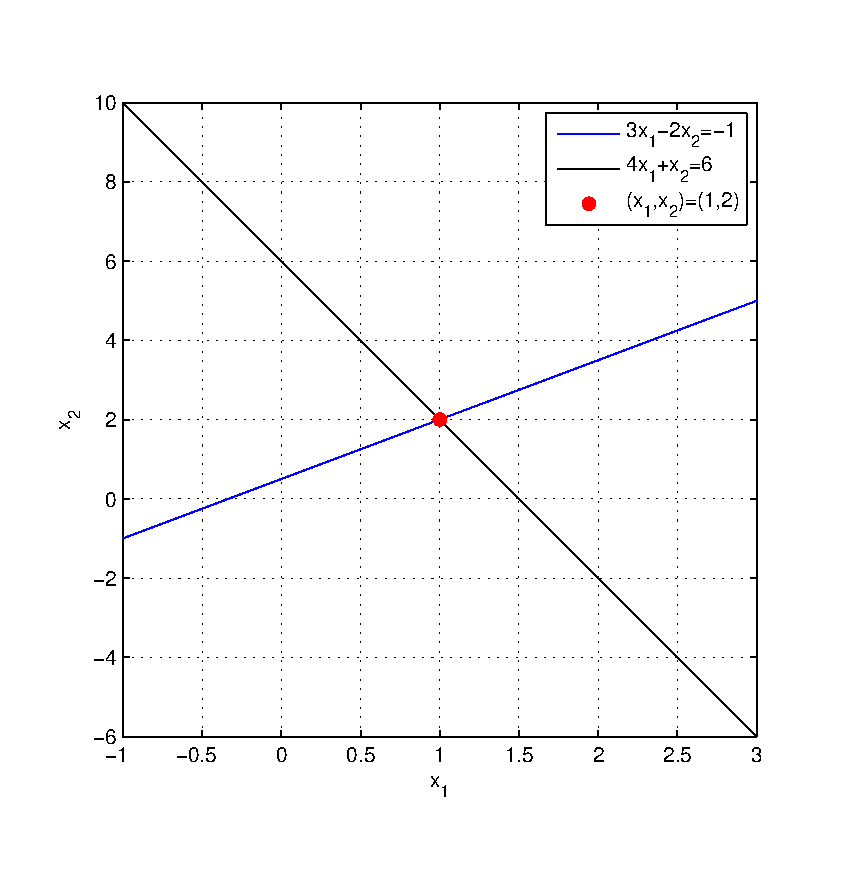
\includegraphics[width=12cm]{recta1}
\bicaption{Sistema de ecuaciones con solución única}{Equation system with unique solution}
\label{fig:recta1}
\end{figure}

\begin{paracol}
    
Supongamos ahora el siguiente sistema, también de dos ecuaciones con dos incógnitas,

\begin{align*}
4x_1+x_2&=6\\
2x_1+\frac{1}{2} x_2&=-1
\end{align*}

El sistema no tiene solución. Su matriz de coeficientes tiene determinante cero, por lo que no es invertible,
\begin{equation*}
\vert A \vert =\begin{vmatrix}
4& 1\\
2& 1/2
\end{vmatrix} =0 \Rightarrow \nexists A^{-1}
\end{equation*}

\switchcolumn
Now suppose the following system, also of two equations with two unknowns,
\begin{align*}
4x_1+x_2&=6\\
2x_1+\frac{1}{2} x_2&=-1
\end{align*}

The system has no solution. Its coefficient matrix has zero determinant, so it is not invertible,
\begin{equation*}
\vert A \vert =\begin{vmatrix}
4& 1\\
2& 1/2
\end{vmatrix} =0 \Rightarrow \nexists A^{-1}
\end{equation*}

\switchcolumn
Si representamos gráficamente las dos ecuaciones de este sistema (figura \ref{fig:recta2}) es fácil entender lo que pasa, las rectas son paralelas, no existe ningún punto $(x_1,x_2)$ que pertenezca a las dos rectas, y por tanto el sistema carece de solución.

\switchcolumn
If we represent graphically the two equations of this system (figure \ref{fig:recta2}) it is easy to understand what happens, the lines are parallel, there is no point $(x_1,x_2)$ that belongs to the two lines, and therefore the system has no solution.

\end{paracol}



\begin{figure}[h]
\centering
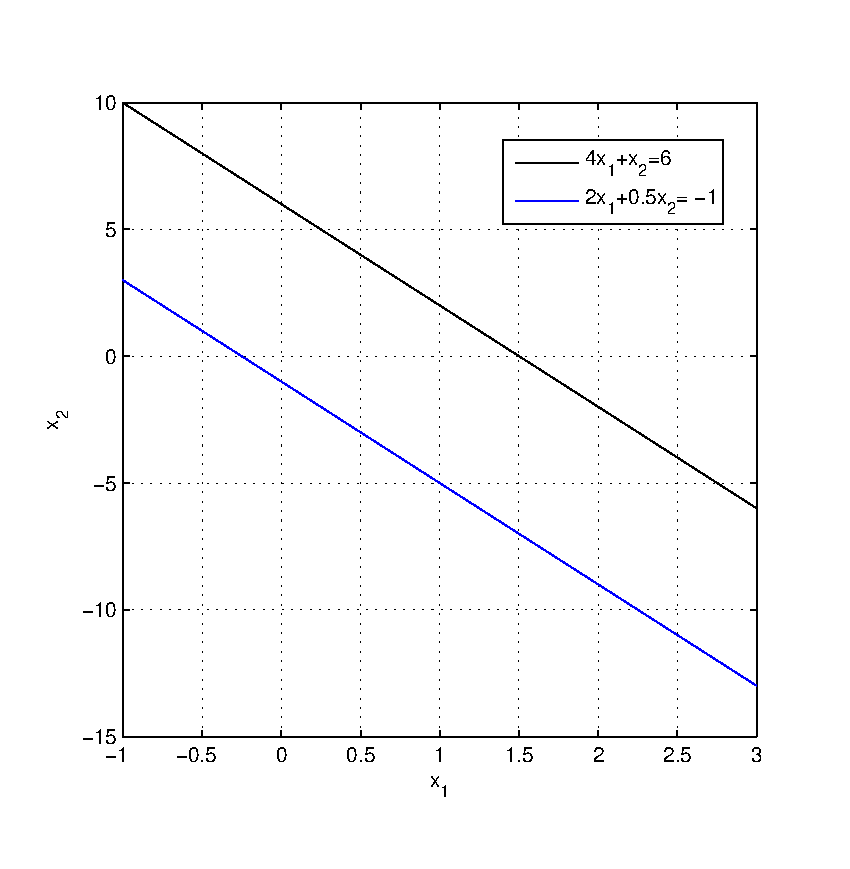
\includegraphics[width=12cm]{recta2}
\bicaption{Sistema de ecuaciones sin solución}{Equation system without solution}
\label{fig:recta2}
\end{figure}

\begin{paracol}{2}
Dos rectas paralelas lo son, porque tienen la misma pendiente. Esto se refleja en la matriz de coeficientes, en que las filas son proporcionales; si multiplicamos la segunda fila por dos, obtenemos la primera. 

\switchcolumn

Two parallel lines are parallel because they have the same slope. This is reflected in the coefficient matrix, where the rows are proportional; if we multiply the second row by two, we get the first row. 

\switchcolumn
Por último, el sistema,

\begin{align*}
4x_1+x_2&=6\\
2x_1+\frac{1}{2} x_2&=3
\end{align*}

posee infinitas soluciones. la razón es que la segunda ecuación es igual que la primera multiplicada por dos: es decir, representa exactamente la misma relación lineal entre las variables $x_1$ y $x_2$, por tanto, todos los puntos de la recta son solución del sistema. De nuevo, la matriz de coeficientes del sistema no tiene inversa ya que su determinante es cero.

\switchcolumn
Finally, the system,

\begin{align*}
4x_1+x_2&=6.
2x_1+frac{1}{2} x_2&=3
\end{align*}

has infinite solutions.The reason is that the second equation is the same as the first equation multiplied by two: that is, it represents exactly the same linear relationship between the variables $x_1$ and $x_2$, therefore, all the points on the line are solutions of the system. Again, the coefficient matrix of the system has no inverse since its determinant is zero.
\end{paracol}

\begin{figure}[h]
\centering
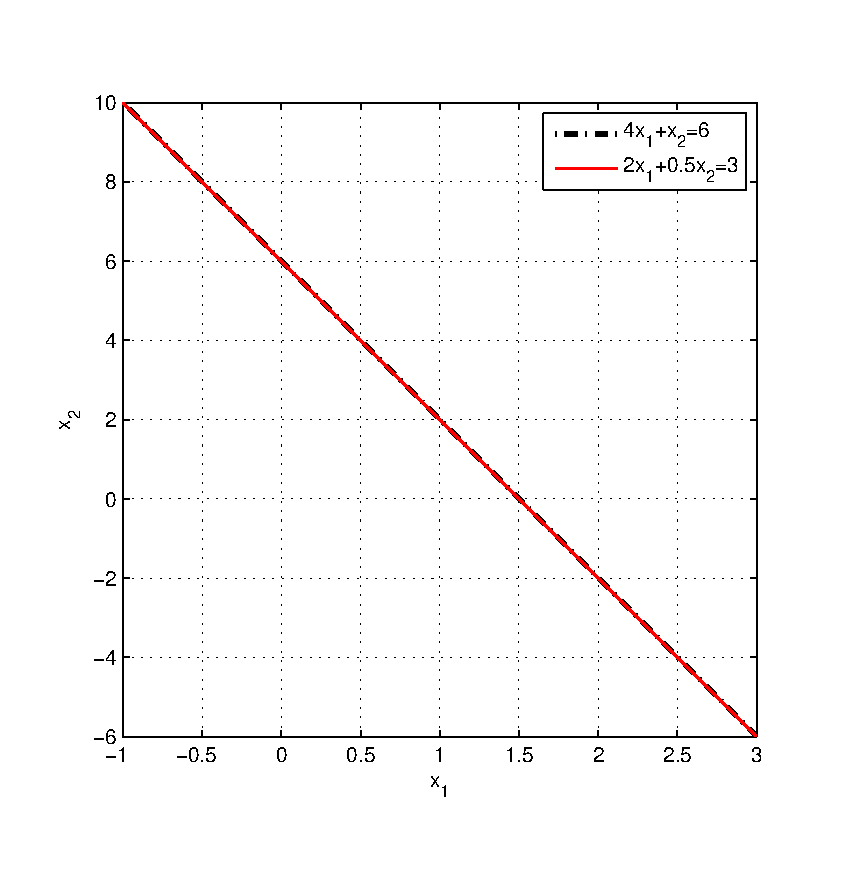
\includegraphics[width=12cm]{recta3.eps}
\bicaption{Sistema de ecuaciones con infinitas soluciones}{Equation system with infinite solutions}
\label{recta3}
\end{figure}

\begin{paracol}{2}
Para sistemas de ecuaciones de dimensión mayor, se cumple también que que el sistema no tiene solución única si el determinante de su matriz de coeficiente es cero. En todos los demás casos, es posible obtener la solución del sistema invirtiendo la matriz de coeficientes y multiplicando el resultado por el vector de términos independientes.

En cuanto un sistema de ecuaciones tiene una dimensión suficientemente grande, invertir su matriz de coeficientes se torna un problema costoso o sencillamente inabordable.

Desde un punto de vista numérico, la inversión de una matriz, presenta frecuentemente problemas debido al error de redondeo en las operaciones. Por esto, casi nunca se resuelven los sistemas de ecuaciones invirtiendo su matriz de coeficientes. A lo largo de este capítulo estudiaremos dos tipos de métodos de resolución de sistemas de ecuaciones. El primero de ellos recibe el nombre genérico de métodos directos, el segundo tipo lo constituyen los llamados métodos iterativos.

\switchcolumn
For higher dimensional systems of equations, it is also true that the system has no unique solution if the determinant of its coefficient matrix is zero. In all other cases, it is possible to obtain the solution of the system by inverting the coefficient matrix and multiplying the result by the vector of independent terms.

As soon as a system of equations has a sufficiently large dimension, inverting its coefficient matrix becomes a costly or simply intractable problem.

From a numerical point of view, the inversion of a matrix often presents problems due to the rounding error in the operations. For this reason, systems of equations are almost never solved by inverting their matrix of coefficients. Throughout this chapter we will study two types of methods for solving systems of equations. The first of these is known generically as direct methods, while the second type is known as iterative methods.

\switchcolumn
\section{Condicionamiento}
En la introducción hemos visto que para que un sistema de ecuaciones tenga solución, es preciso que su matriz de coeficientes sea invertible. Sin embargo cuando tratamos de resolver un sistema de ecuaciones numéricamente, empleando un ordenador, debemos antes examinar cuidadosamente la matriz de coeficientes del sistema. Veamos un ejemplo: el sistema,

\begin{align*}
4x_1+x_2&=6\\
2x_1+0.4 x_2&=-1
\end{align*}

\switchcolumn
\section{Condition number}
In the introduction we have seen that for a system of equations to have a solution, its coefficient matrix must be invertible. However, when we try to solve a system of equations numerically, using a computer, we must first carefully examine the matrix of coefficients of the system. Let us look at an example: the system,

\begin{align*}
4x_1+x_2&=6\\
2x_1+0.4 x_2&=-1
\end{align*}

\switchcolumn

Tiene como soluciones,
\begin{equation*}
x=\begin{pmatrix}
-8.5\\
40
\end{pmatrix}
\end{equation*}

\switchcolumn
 Has the following solutions,
 \begin{equation*}
x=\begin{pmatrix}
-8.5\\
40
\end{pmatrix}
\end{equation*}

\switchcolumn

Si alteramos ligeramente uno de sus coeficientes,

\begin{align*}
4x_1+x_2&=6\\
2x_1+0.4{\color{red}9} x_2&=-1
\end{align*}

\switchcolumn

If we slightly change one of the coefficients,
\begin{align*}
4x_1+x_2&=6\\
2x_1+0.4{\color{red}9} x_2&=-1
\end{align*}

\switchcolumn

Las soluciones se alteran bastante;  se vuelven aproximadamente 10 veces más grande,
\begin{equation*}
x=\begin{pmatrix}
-98.5\\
400
\end{pmatrix}
\end{equation*}

\switchcolumn

The solutions become quite altered; they become about 10 times larger,
\begin{equation*}
x=\begin{pmatrix}
-98.5\\
400
\end{pmatrix}
\end{equation*}

\switchcolumn
y si volvemos a alterar el mismo coeficiente,

\begin{align*}
4x_1+x_2&=6\\
2x_1+0.4{\color{red}99} x_2&=-1
\end{align*}

\switchcolumn

if we change again the same coefficient,

\begin{align*}
4x_1+x_2&=6\\
2x_1+0.4{\color{red}99} x_2&=-1
\end{align*}

\switchcolumn

La solución es aproximadamente 100 veces más grande,
\begin{equation*}
x=\begin{pmatrix}
-998.5\\
4000
\end{pmatrix}
\end{equation*}

\switchcolumn

The solution is about 100 times larger,

\begin{equation*}
x=\begin{pmatrix}
-998.5\\
4000
\end{pmatrix}
\end{equation*}

\switchcolumn
La razón para estos cambios es fácil de comprender intuitivamente; a medida que aproximamos el coeficiente a $0.5$, estamos haciendo que las dos ecuaciones lineales sean cada vez mas paralelas, pequeñas variaciones en la pendiente, modifican mucho la posición del punto de corte.

Cuando pequeñas variaciones en la matriz de coeficientes generan grandes variaciones en las soluciones del sistema, se dice que el sistema está mal condicionado, en otras palabras: que no es un sistema bueno para ser resuelto numéricamente. Las soluciones obtenidas para un sistema mal condicionado, hay que tomarlas siempre con bastante escepticismo.

Para estimar el buen o mal condicionamiento de un sistema, se emplea el número de condición, que definimos en el capítulo \ref{ch:numpy} en la sección \ref{sec:SVD}, al hablar de la factorización SVD. El número de condición de una matriz es el cociente entre sus valores singulares mayor y menor.  Cuanto más próximo a $1$ sea el número de condición, mejor condicionada estará la matriz y cuanto mayor sea el número de condición peor condicionada estará.

\switchcolumn
The reason for these changes is easy to understand intuitively; as we bring the coefficient closer to $0.5$, we are making the two linear equations more and more parallel, and small variations in the slope greatly modify the position of the cut-off point.

When small variations in the matrix of coefficients generate large variations in the solutions of the system, it is said that the system is ill-conditioned, in other words: that it is not a good system to be solved numerically. The solutions obtained for an ill-conditioned system must always be taken with considerable scepticism.

To estimate the good or bad conditioning of a system, we use the condition number, which we defined in the chapter \ref{ch:numpy} in section \ref{sec:SVD}, when talking about SVD factorisation. The condition number of a matrix is the quotient of its largest and smallest singular values.  The closer the condition number is to $1$, the better conditioned the matrix is, and the larger the condition number, the worse conditioned it is.

\switchcolumn

En Python dentro del paquete \texttt{linalg} de \texttt{numpy} está la función \texttt{cond} que nos permite obtener el número de condición de una matriz. Si lo aplicamos a la matriz de coeficientes del último ejemplo mostrado,

\switchcolumn
In Python, we can use the function \texttt{cond} inside the \texttt{linalg} module in \texttt{numpy} to compute the condition number of a matrix. We can apply to the last example coefficient matrix

\end{paracol}

\begin{verbatim}
>> A=[4 1; 2, 0.499]

A =

    4.0000    1.0000
    2.0000    0.4990

>> nc=cond(A)

nc =

  5.3123e+003
\end{verbatim}

El número está bastante alejado de uno, lo que, en principio, indica un mal condicionamiento del sistema. 

Incidentalmente, podemos calcular la factorización svd de la matriz de coeficientes y dividir el valor singular mayor entre el menor para comprobar que el resultado es el mismo que nos da la función \texttt{cond},
\begin{verbatim}
>> [U,S,V]=svd(A)

U =

   -0.8944   -0.4472
   -0.4472    0.8944


S =

    4.6097         0
         0    0.0009


V =

   -0.9702    0.2424
   -0.2424   -0.9702

>> nc=S(1,1)/S(2,2)

nc =

  5.3123e+003
\end{verbatim}

Matlab emplea también la función \texttt{rnc=rcond(A)} para estimar el condicionamiento de una matriz. No describiremos el método, simplemente diremos que en lugar de obtener un número de condición para la matriz, se utiliza un valor recíproco. De este modo, cuanto más se aproxima a uno el resultado de \texttt{rcond}, mejor condicionada está la matriz, y cuanto más se aproxime a cero peor. Para nuestro ejemplo anterior,

\begin{verbatim}
>> rnc=rcond(A)

rnc =

  1.3333e-004

\end{verbatim}

Próximo a cero, lo que indica un mal condicionamiento de $A$. Nótese que el resultado de \texttt{rcond}, no es el inverso del valor de \texttt{cond}.

\section{Métodos directos}
\subsection{Sistemas triangulares}
Vamos a empezar el estudio de los métodos directos por los algoritmos de resolución de los sistemas más simples posibles, aquellos cuya matriz de coeficientes es una matriz diagonal, triangular superior o triangular inferior.
\paragraph{Sistemas diagonales.} Un sistema diagonal es aquel cuya matriz de coeficientes es una matriz diagonal. 

\begin{equation*}
\left. \begin{aligned}
a_{11}&x_1=b_1\\
a_{22}&x_2=b_2\\
\cdots & \\
a_{nn}&x_n=b_n
\end{aligned}\right\} \Rightarrow	\overbrace{\begin{pmatrix}
a_{11}& 0& \cdots & 0\\
0& a_{22}& \cdots & 0\\
\vdots & \vdots & \ddots & \vdots\\
0& 0& \cdots & a_{nn}
\end{pmatrix}}^A \cdot \overbrace{\begin{pmatrix}
x_1\\
x_2\\
\vdots \\
x_n
\end{pmatrix}}^x=\overbrace{\begin{pmatrix}
b_1\\
b_2\\
\vdots \\
b_n
\end{pmatrix}}^b
\end{equation*}

Su resolución es trivial, basta dividir cada término independiente por el elemento correspondiente de la diagonal de la matriz de coeficientes,
\begin{equation*}
x_i=\frac{b_i}{a_{ii}}
\end{equation*}

Para obtener la solución basta crear en Matlab un sencillo bucle \texttt{for},
\begin{verbatim}
n=size(A,1);
x=zeros(n,1);
for i=1:n
    x(i)=b(i)/A(i,i);
end
\end{verbatim} 

\paragraph{Sistemas triangulares inferiores: método de sustituciones progresivas.} Un sistema triangular inferior de $n$ ecuaciones con $n$ incógnitas tendrá la forma general,

\begin{equation*}
\left. \begin{aligned}
a_{11}&x_1=b_1\\
a_{21}&x_1+a_{22}x_2=b_2\\
\cdots & \\
a_{n1}&x_1+a_{n2}x_2+\cdots +a_{nn}x_n=b_n
\end{aligned}\right\} \Rightarrow	\overbrace{\begin{pmatrix}
a_{11}& 0& \cdots & 0\\
a_{21}& a_{22}& \cdots & 0\\
\vdots & \vdots & \ddots & \vdots\\
a_{n1}& a_{n2}& \cdots & a_{nn}
\end{pmatrix}}^A \cdot \overbrace{\begin{pmatrix}
x_1\\
x_2\\
\vdots \\
x_n
\end{pmatrix}}^x=\overbrace{\begin{pmatrix}
b_1\\
b_2\\
\vdots \\
b_n
\end{pmatrix}}^b
\end{equation*}

El procedimiento para resolverlo a \emph{mano} es muy sencillo,
despejamos la primera la primera incógnita de la primera ecuación,
\begin{equation*}
x_1=\frac{b_1}{a_{11}}
\end{equation*}

A continuación sustituimos este resultado en la segunda ecuación, y despejamos $x_2$,
\begin{equation*}
x_2=\frac{b_2-a_{21}x_1}{a_{22}}
\end{equation*}

De cada ecuación vamos obteniendo una componente del vector solución, sustituyendo las soluciones obtenidas en las ecuaciones anteriores, así cuando llegamos a la ecuación $i$,

\begin{equation*}
x_i=\frac{b_i-\sum_{j=1}^{i-1}a_{ij}x_j}{a_{ii}}
\end{equation*}

Si repetimos este mismo proceso hasta llegar a la última ecuación del sistema, $n$, habremos obtenido la solución completa.

EL siguiente código calcula la solución de un sistema triangular inferior mediante sustituciones progresivas,

\begin{lstlisting}
function x = progresivas(A,b)
% Esta Función permite obtener la solucion de un sistema triangular inferior
% empleando sustituciones progresivas. La variables de entrada son la matriz
% de coeficientes A  y el vector de terminos independientes b. la solucion se
% devuelve como un vector columna en la varible x

%%%%%%%%%%%%%%%%%%%%%%%%%%%%%%%%%%%%%%%%%%%

% Obtenemos el tamaño de la matriz de coeficientes y comprobamos que es
% cuadrada,
[f,c]=size(A);
if f~=c
    error('la matriz de coeficientes no es cuadrada')
end
% construimos un vector solucion, inicialmente formado por ceros,
x=zeros(f,1);
% construimos un bucle for para ir calculando progresivamente las soluciones
% del sistema
for i=1:f
    % primero igualamos la solución al termino independiente de la ecuación
    % que toque...
    x(i)=b(i)
    % y luego creamos un bucle para ir restando todas las soluciones
    % anteriores...
    for j=1:i-1
    x(i)=x(i)-A(i,j)*x(j)
    end
    % para terminar dividimos por el elemento de la diagonal de la matriz de
    % coeficientes...
    x(i)=x(i)/A(i,i)
end
\end{lstlisting}

\paragraph{Sistemas triangulares superiores: método de sustituciones regresivas.} En este caso, el sistema general de $n$ ecuaciones con $n$ incógnitas tendrá la forma general,

\begin{equation*}
\left. \begin{aligned}
a_{11}x_1+a_{12}x_2+\cdots +a_{1n}x_n=b_1\\
a_{22}x_2+\cdots +a_{2n}x_n=b_2\\
\cdots  \\
a_{nn}x_n=b_n
\end{aligned}\right\} \Rightarrow	\overbrace{\begin{pmatrix}
a_{11}& a_{12}& \cdots & a_{1n}\\
0& a_{22}& \cdots & a_{2n}\\
\vdots & \vdots & \ddots & \vdots\\
0& 0& \cdots & a_{nn}
\end{pmatrix}}^A \cdot \overbrace{\begin{pmatrix}
x_1\\
x_2\\
\vdots \\
x_n
\end{pmatrix}}^x=\overbrace{\begin{pmatrix}
b_1\\
b_2\\
\vdots \\
b_n
\end{pmatrix}}^b
\end{equation*}


El método de resolución es idéntico al de un sistema triangular inferior, simplemente que ahora, empezamos a resolver por la última ecuación,
\begin{equation*}
x_n=\frac{b_n}{a_{nn}}
\end{equation*}
Y seguimos sustituyendo hacia arriba,
\begin{equation*}
x_{n-1}=\frac{b_{n-1}-a_{(n-1)n}x_{n}}{a_{(n-1)(n-1)}}
\end{equation*}

\begin{equation*}
x_i=\frac{b_i-\sum_{j=i+1}^{n}a_{ij}x_j}{a_{ii}}
\end{equation*}

El código para implementar este método es similar al de las sustituciones progresivas. Se deja como ejercicio el construir una función en Matlab que calcule la solución de un sistema triangular superior por el método de las sustituciones regresivas.


\subsection{Métodos basados en las factorizaciones}
Puesto que sabemos como resolver sistemas triangulares, una manera de resolver sistemas más complejos sería encontrar métodos para reducirlos a sistemas triangulares. De este modo evitamos invertir la matriz de coeficientes y los posibles problemas de estabilidad numérica derivados de dicha operación. En el capítulo anterior \ref{sec:fact}, vimos varios métodos de factorizar una matriz, que permiten una aplicación directa a la resolución de sistemas.
\paragraph{Factorización LU.} En el capítulo anterior \ref{sec:LU} vimos como factorizar una matriz en el producto de dos, una triangular inferior $L$ y una triangular superior $U$. La factorización podía incluir pivoteo de filas, para alcanzar una solución numéricamente estable. En este caso la factorización LU tomaba la forma,
\begin{equation*}
P\cdot A = L\cdot U
\end{equation*}

Donde $P$ representa una matriz de permutaciones.

Supongamos que queremos resolver un sistema de $n$ ecuaciones lineales con $n$ incógnitas que representamos genéricamente en forma matricial, como siempre,
\begin{equation*}
A\cdot x=b
\end{equation*}

Si calculamos la fatorización LU de su matriz de  coeficientes,

\begin{equation*}
A \rightarrow P\cdot A = L\cdot U
\end{equation*}

Podemos transformar nuestro sistema de ecuaciones en uno equivalente aplicando la matriz de permutaciones, por la izquierda, a ambos lados del igual. El efecto es equivalente a que cambiáramos el orden en que se presentan las ecuaciones del sistema,

\begin{equation*}
A\cdot x=b\rightarrow P\cdot A \cdot x=P\cdot b
\end{equation*}

Si sustituimos ahora $P\cdot A$ por su factorización LU,

\begin{equation*}
P\cdot A \cdot x=P\cdot b \rightarrow L\cdot U \cdot x= P\cdot b
\end{equation*}

El nuevo sistema puede resolverse en dos pasos empleando sustituciones regresivas y sustituciones progresivas. Para ello, asociamos el producto $U\cdot x$, a un vector de incógnitas auxiliar al que llamaremos $z$,

\begin{equation*}
U\cdot x=z
\end{equation*}

Si sustituimos nuestro vector auxiliar $z$ en la expresión matricial de nuestro sistema de ecuaciones,

\begin{equation*}
L\cdot \overbrace{U\cdot x}^z=P\cdot b \rightarrow L\cdot z=P\cdot b
\end{equation*}

El sistema resultante es triangular inferior, por lo que podemos resolverlo por sustituciones progresivas, y obtener de este modo los valores de $z$. Podemos finalmente obtener la solución del sistema a través de la definición de $z$; $U\cdot x =z$, se trata de un sistema triangular superior, que podemos resolver mediante sustituciones regresivas.

Veamos un ejemplo. Supongamos que queremos resolver el sistema de ecuaciones lineales,

\begin{equation*}
\begin{pmatrix}
1& 3& 2\\
2& -1& 1\\
1& 4& 3
\end{pmatrix}\cdot \begin{pmatrix}
x_1\\
x_2\\
x_3
\end{pmatrix}=\begin{pmatrix}
13\\
3\\
18
\end{pmatrix}
\end{equation*}

En primer lugar deberíamos comprobar que la matriz de coeficiente esta bien condicionada,
\begin{verbatim}
>> A=[1 3 2;2 -1 1;1 4 3]
A =

     1     3     2
     2    -1     1
     1     4     3
>> nc=cond(A)
nc =

   24.3827
\end{verbatim}
No es un valor grande, con lo que podemos considerar que $A$ está bien condicionada. 
Calculamos la factorización LU de la matriz de coeficientes, para ello podemos emplear el programa lufact.m, incluido en el capítulo anterior \ref{lufact}, o bien la función \texttt{lu} de Matlab,

\begin{verbatim}
>> [L U P]=lufact(A)

L =

    1.0000         0         0
    0.5000    1.0000         0
    0.5000    0.7778    1.0000

U =

    2.0000   -1.0000    1.0000
         0    4.5000    2.5000
         0         0   -0.4444

P =

     0     1     0
     0     0     1
     1     0     0
\end{verbatim}

A continuación debemos aplicar la matriz de permutaciones, al vector de términos independientes del sistema, para poder construir el sistema equivalente $L\cdot U=P\cdot b$,
\begin{verbatim}
>> b=[13;3;18]

b =

    13
     3
    18

>> bp=P*b

bp =

     3
    18
    13

\end{verbatim}

Empleamos la matriz $L$ obtenida y el producto $bp=P\cdot b$ que acabamos de calcular, para obtener, por sustituciones progresivas, el vector auxiliar $z$ descrito más arriba. Empleamos para ello la función \texttt{progresivas}, cuyo código incluimos en la sección anterior, 
\begin{verbatim}
>> z=progresivas(L,bp)
z =

    3.0000
   16.5000
   -1.3333
\end{verbatim}

Finalmente, podemos obtener la solución del sistema sin más que aplicar el método de las sustituciones regresiva a la matriz $U$ y al vector auxiliar $z$ que acabamos de obtener,\footnote{La función \texttt{regresivas} no se ha suministrado ni existe en Matlab. Su construcción se ha dejado como ejercicio en la sección anterior.}

\begin{verbatim}
>> x=regresivas(U,z)
x =

    1.0000
    2.0000
    3.0000


\end{verbatim}
Para comprobar que la solución es correcta basta multiplicar la matriz de coeficientes del sistema original por el resultado obtenido para $x$ y comprobar que obtenemos como resultado el vector de términos independientes.
\begin{verbatim}
>> A*x

ans =

    13
     3
    18
\end{verbatim}
 
\paragraph{Factorización de Cholesky.} Como vimos en el capitulo anterior \ref{chol}, la factorización de Cholesky permite descomponer una matriz $A$ en el producto de de una matriz triangular inferior, por su traspuesta. 
\begin{equation*}
A=L\cdot L^T
\end{equation*}
Para ello, es preciso que $A$ sea simétrica y definida positiva (ver \ref{tiposm}). 

Por tanto, en el caso particular de un sistema cuya matriz de coeficientes fuera simétrica y definida positiva, podríamos descomponerla empleando la factorización de Cholesky y resolver el sistema de modo análogo a como hicimos con con la factorización LU, sustituimos $A$ por el producto $L\cdot L^T$,
\begin{equation*}
A\cdot x = b \rightarrow L\cdot L^T\cdot x= b
\end{equation*}

Definimos el vector auxiliar $z$,
\begin{equation*}
L^T\cdot x= z
\end{equation*}

Resolvemos por sustituciones progresivas el sistema,

\begin{equation*}
L\cdot z=b
\end{equation*}

y por último obtenemos $x$ resolviendo por sustituciones regresivas el sistema,

\begin{equation*}
L^T\cdot x=z
\end{equation*}

La siguiente secuencia de comandos de Matlab muestra la resolución del sistema,
\begin{equation*}
\begin{pmatrix}
2& 5& 1\\
5& 14& 2\\
1& 2& 6
\end{pmatrix}\cdot \begin{pmatrix}
x_1\\
x_2\\
x_3
\end{pmatrix}=\begin{pmatrix}
15\\
39\\
23
\end{pmatrix}
\end{equation*}

\begin{verbatim}
>> A=[2 5 1;5 14 2;1 2 6]
A =
     2     5     1
     5    14     2
     1     2     6

>> b=[15;39;23]
b =
    15
    39
    23

>> L=cholesky(A)
L =
    1.4142         0         0
    3.5355    1.2247         0
    0.7071   -0.4082    2.3094

>> z=progresivas(L,b)
z =
   10.6066
    1.2247
    6.9282

>> x=regresivas(L',z)
x =
    1.0000
    2.0000
    3.0000

>> A*x
ans =
    15
    39
    23
\end{verbatim}

En este ejemplo se ha empleado la función \texttt{cholesky}, cuyo código se incluyó en el capítulo anterior \ref{chol}, para factorizar la matriz de coeficientes del sistema. La factorización se podría haber llevado a cabo igualmente, empleando la función de Matlab \texttt{chol}\footnote{Matlab, por defecto, devuelve una matriz triangular superior: \texttt{U = chol(A)}. La factorización es la misma que la descrita en este apartado. Simplemente $L^T = U$ y $L = U^T$. Por tanto, si se emplea directamente el comando \texttt{chol}   de matlab: $A\cdot x = b \rightarrow U^T\cdot U\cdot x= b$}

\paragraph{Factorización QR} Como vimos en el capítulo anterior \ref{QR}, la factorización QR, descompone una matriz en el producto de una matriz ortogonal  (ver \ref{tiposm}) $Q$  por una matriz triangular superior $R$. Si obtenemos la factorización QR de la matriz de coeficientes de un sistema,

\begin{equation*}
A\cdot x=b \rightarrow Q\cdot R\cdot x =b
\end{equation*}

Podemos resolver ahora el sistema en dos pasos. En primer lugar, como Q es ortogonal, $Q^{-1}=Q^T$, podemos multiplicar por $Q^T$ a ambos lados de la igualdad,

\begin{equation*}
Q\cdot R\cdot x =b \rightarrow Q^T\cdot Q\cdot R\cdot x = Q^T \cdot b \rightarrow R\cdot x= Q^T\cdot b
\end{equation*}

Pero el sistema resultante, es un sistema triangular superior, por lo que podemos resolverlo por sustituciones regresivas. Tomando el mismo ejemplo que resolvimos antes por factorización LU,

\begin{equation*}
\begin{pmatrix}
1& 3& 2\\
2& -1& 1\\
1& 4& 3
\end{pmatrix}\cdot \begin{pmatrix}
x_1\\
x_2\\
x_3
\end{pmatrix}=\begin{pmatrix}
13\\
3\\
18
\end{pmatrix}
\end{equation*}

podemos ahora resolverlo mediante factorización QR. Para ello aplicamos la función \texttt{QRF2} incluida en el capítulo anterior \ref{QR}, o directamente la función de Matlab \texttt{qr}, a la matriz de coeficientes del sistema,

\begin{verbatim}
>> A=[1 3 2;2 -1 1;1 4 3]
A =
     1     3     2
     2    -1     1
     1     4     3

>> [Q,R]=QRF2(A)
Q =
    0.4082    0.4637   -0.7863
    0.8165   -0.5707    0.0874
    0.4082    0.6777    0.6116

R =
    2.4495    2.0412    2.8577
         0    4.6726    2.3898
         0         0    0.3495
\end{verbatim}

A continuación multiplicamos $Q^T$ por el vector de términos independientes,

\begin{verbatim}
>> b=[13;3;18]
b =
    13
     3
    18

>> z=Q'*b
z =
   15.1052
   16.5147
    1.0484
\end{verbatim}

Por último resolvemos el sistema $R\cdot x= Q^T\cdot b$ mediante sustituciones regresivas y comprobamos el resultado,

\begin{verbatim}
>> x=regresivas(R,z)

x =

    1.0000
    2.0000
    3.0000

>> A*x

ans =

   13.0000
    3.0000
   18.0000
\end{verbatim}

\paragraph{Factorización SVD.} La  factorización svd \ref{sec:SVD}, descompone una matriz cualquiera en el producto de tres matrices,
\begin{equation*}
A=U\cdot S\cdot V^T
\end{equation*}
Donde $U$ y $V$ son matrices ortogonales y S es una matriz diagonal. Si calculamos la factorización svd de la matriz de coeficiente de un sistema,

\begin{equation*}
A\cdot x=b \rightarrow U\cdot S\cdot V^T\cdot x=b
\end{equation*}

Como en el caso de la factorización QR, podemos aprovechar la ortogonalidad de las matrices $U$ y $V$ para simplificar el sistema,

\begin{equation*}
U\cdot S\cdot V^T\cdot x=b \rightarrow U^T\cdot U\cdot S\cdot V^T \cdot x= U^T\cdot b \rightarrow S\cdot V^T \cdot x=U^T\cdot b
\end{equation*}

Como en casos anteriores, podemos crear un vector auxiliar $z$,
\begin{equation*}
V^T\cdot x=z
\end{equation*}

de modo que resolvemos primero el sistema,
\begin{equation*}
S\cdot z= U^T\cdot b
\end{equation*}

Como la matriz $S$ es diagonal, se trata de un sistema diagonal que, como hemos visto, es trivial de resolver.

Una vez conocido $Z$ podemos obtener la solución del sistema original, haciendo ahora uso de la ortogonalidad de la matriz $V$,

\begin{equation*}
V^T\cdot x=z \rightarrow V\cdot V^T\cdot x=V\cdot z \rightarrow x=V\cdot z
\end{equation*}

Volvamos a nuestro ejemplo,
\begin{equation*}
\begin{pmatrix}
1& 3& 2\\
2& -1& 1\\
1& 4& 3
\end{pmatrix}\cdot \begin{pmatrix}
x_1\\
x_2\\
x_3
\end{pmatrix}=\begin{pmatrix}
13\\
3\\
18
\end{pmatrix}
\end{equation*}

En primer lugar factorizamos la matriz de coeficientes empleando el comando \texttt{svd} de Matlab,

\begin{verbatim}
>> A=[1 3 2;2 -1 1;1 4 3]
A =

     1     3     2
     2    -1     1
     1     4     3

>> [U,S,V]=svd(A)
U =

   -0.5908   -0.0053   -0.8068
   -0.0411   -0.9985    0.0366
   -0.8058    0.0548    0.5897

S =

    6.3232         0         0
         0    2.4393         0
         0         0    0.2593


V =

   -0.2339   -0.7983   -0.5549
   -0.7835    0.4927   -0.3786
   -0.5757   -0.3463    0.7408

\end{verbatim}

Calculamos a continuación el valor del vector auxiliar $z$,

\begin{verbatim}
>> ba=U'*b
ba =
  -22.3076
   -2.0777
    0.2360

>> z=S^-1*ba
z =
   -3.5279
   -0.8518
    0.9101
\end{verbatim}
por último, calculamos $x$ y comprobamos la solución obtenida,

\begin{verbatim}
>> x=V*z
x =
    1.0000
    2.0000
    3.0000

>> A*x
ans =
   13.0000
    3.0000
   18.0000
\end{verbatim}

\subsection{El método de eliminación de Gauss.}\index{Gauss! Método de eliminación gaussiana} El método de eliminación gaussiana es el mismo descrito en el capítulo anterior \ref{sec:LU} para obtener la matriz triangular superior $U$ en la factorización LU de una matriz. Como ya se explicó en detalle, el método consiste en \emph{hacer  cero} todos los elementos situados por debajo de la diagonal de una matriz. Para ello se sustituyen progresivamente las filas de la matriz, exceptuando la primera, por combinaciones adecuadas de dicha fila con las anteriores.

Toda la discusión incluida en el capítulo anterior sobre la eliminación de Gauss, es válida también para la resolución de sistemas, por lo que no volveremos a repetirla. Nos centraremos solo en su aplicación al problema de resolver un sistema de ecuaciones lineales.
===========Traido del capituilo anterior=============================
Uno de los métodos más empleados para calcular la factorización LU de una matriz, se basa en el método conocido como eliminación gaussiana. La idea es convertir en ceros los elementos situados por debajo de la diagonal de la matriz. Para ello, se sustituyen progresivamente las filas de la matriz, exceptuando la primera, por combinaciones  formadas con la fila que se sustituye y la fila anterior.
 veamos en qué consiste con un ejemplo. Supongamos que tenemos la siguiente matriz de orden $4 \times 4$, 

\begin{equation*}
A=\begin{pmatrix}
3& 4& 2&5\\
2& 0& 1& -2\\
3& 2& 1& 8\\
5& 2& 3& 2
\end{pmatrix} 
\end{equation*}

Si sustituimos la segunda fila por el resultado de restarle la primera multiplicada por $2$ y dividida por $3$ obtendríamos la matriz,

\begin{equation*}
A=\begin{pmatrix}
3& 4& 2&5\\
2& 0& 1& -2\\
3& 2& 1& 8\\
5& 2& 3& 2
\end{pmatrix} \rightarrow [2\ 0\ 1\ -2]-\frac{2}{3} [3\ 4\ 2\ 5] \rightarrow U_1=\begin{pmatrix}
3& 4& 2&5\\
0& -2.6& -0.33& -5.33\\
3& 2& 1& 8\\
5& 2& 3& 2
\end{pmatrix}
\end{equation*}

De modo análogo, si sustituimos ahora la tercera fila por el resultado de restarle la primera multiplicada por $3$ y dividida $3$,
 
\begin{equation*}
U_1=\begin{pmatrix}
3& 4& 2&5\\
0& -2.6& -0.33& -5.33\\
3& 2& 1& 8\\
5& 2& 3& 2
\end{pmatrix} \rightarrow [3\ 2\ 1\ 8]-\frac{3}{3} [3\ 4\ 2\ 5] \rightarrow U_1=\begin{pmatrix}
3& 4& 2&5\\
0& -2.6& -0.33& -5.33\\
0& -2& -1& -3\\
5& 2& 3& 2
\end{pmatrix}
\end{equation*}

Por último si sustituimos la última fila por el resultado de restarle la primera multiplicada por $5$ y dividida por $3$,

\begin{equation*}
U_1=\begin{pmatrix}
3& 4& 2&5\\
0& -2.6& -0.33& -5.33\\
0& -2& -1& -3\\
5& 2& 3& 2
\end{pmatrix} \rightarrow [5\ 2\ 3\ 2]-\frac{5}{3} [3\ 4\ 2\ 5] \rightarrow U_1=\begin{pmatrix}
3& 4& 2&5\\
0& -2.6& -0.33& -5.33\\
0& -2& -1& -3\\
0& -4,66& -0.33& -6.33
\end{pmatrix}
\end{equation*}

El resultado que hemos obtenido, tras realizar esta transformación , es una nueva matriz $U$ en la que todos los elementos de su primera columna, por debajo de la diagonal, son ceros.

Podemos proceder de modo análogo para \emph{eliminar} ahora los elementos de la segunda columna situados por debajo de la diagonal. Para ellos sustituimos la tercera fila  por la diferencia entre ella y las segunda fila multiplicada por 	$-2$  y dividida por $-2.6$.

\begin{align*}
U_1 &=\begin{pmatrix}
3& 4& 2&5\\
0& -2.6& -0.33& -5.33\\
0& -2& -1& -3\\
0& -4,66& -0.33& -6.33
\end{pmatrix} \rightarrow [0\ -2\ -1\ -3]-\frac{-2}{-2.6} [0\ -2.6\ -0.33\ -5.33\ ] \rightarrow \\
 U_2 &=\begin{pmatrix}
3& 4& 2&5\\
0& -2.6& -0.33& -5.33\\
0& 0& -0.75& 7\\
0& -4.66& -0.33& -6.33
\end{pmatrix}
\end{align*}

Y sustituyendo la última fila por  la diferencia entre ella y la segunda multiplicada por $-4.66$ y dividida por $-2.6$,

\begin{align*}
U_2 &=\begin{pmatrix}
3& 4& 2&5\\
0& -2.6& -0.33& -5.33\\
0& -2& -1& -3\\
0& -4,66& -0.33& -6.33
\end{pmatrix} \rightarrow [0\ -4.66\ -0.33\ -6.33]-\frac{-4.66}{-2.6} [0\ -2.6\ -0.33\ -5.33\ ] \rightarrow \\
 U_2 &=\begin{pmatrix}
3& 4& 2&5\\
0& -2.6& -0.33& -5.33\\
0& 0& -0.75& 7\\
0& 0& 0.25& 3
\end{pmatrix}
\end{align*}

De este modo, los elementos de la segunda columna situados debajo de la diagonal, han sido sustituidos por ceros. Un último paso, nos llevará hasta una matriz triangular superior; sustituimos la última fila por la diferencia entre ella y la tercera fila multiplicada por $0.25$ y dividida por $-0.75$,

\begin{align*}
 U_2 &=\begin{pmatrix}
3& 4& 2&5\\
0& -2.6& -0.33& -5.33\\
0& 0& -0.75& 7\\
0& 0& 0.25& 3
\end{pmatrix} \rightarrow [0\ 0\ 0.25\ 3]-\frac{0.25}{-0.75} [0\ 0\ -0.75\ 7\ ] \rightarrow \\
 U_3 &=\begin{pmatrix}
3& 4& 2&5\\
0& -2.6& -0.33& -5.33\\
0& 0& -0.75& 7\\
0& 0& 0& 5.33
\end{pmatrix}=U
\end{align*}

Podemos ahora, a partir del ejemplo, deducir un procedimiento general. Para \emph{eliminar} ---convertir en 0--- el elemento $a_{ij}$ situado por debajo de la diagonal principal,  $i>j$:
\begin{enumerate}
\item Dividimos los elementos de la fila $j$ por el elemento de dicha fila que a su vez pertenece a la diagonal, $a_{jj}$
\begin{equation*}
\begin{bmatrix}
0/ a_{jj}& 0/ a_{jj}& \cdots & a_{jj}/ a_{jj}& a_{jj+1}/ a_{jj}& \cdots
\end{bmatrix}
\end{equation*}

\item Multiplicamos el resultado de la operación anterior por el elemento $a_{ij}$,
\begin{equation*}
\begin{bmatrix}
a_{ij} \cdot 0/ a_{jj}& a_{ij} \cdot 0/ a_{jj}& \cdots & a_{ij} \cdot a_{jj}/ a_{jj}& a_{ij} \cdot a_{jj+1}/ a_{jj}& \cdots
\end{bmatrix}
\end{equation*}
\item Finalmente, sustituimos la fila $i$ de la matriz de partida por la diferencia  entre ella y el resultado de la operación anterior.
\begin{equation*}
\begin{bmatrix}
0& 0& \cdots& a_{ij}& a_{ij+1}& \cdots
\end{bmatrix}-\begin{bmatrix}
a_{ij} \cdot 0/ a_{jj}& a_{ij} \cdot 0/ a_{jj}& \cdots & a_{ij} \cdot a_{jj}/ a_{jj}& a_{ij} \cdot a_{jj+1}/ a_{jj}& \cdots
\end{bmatrix}
\end{equation*}
\end{enumerate}

Este procedimiento se aplica iterativamente empezando en por el elemento  $a_{21}$ de la matriz y desplazando el cómputo hacia abajo, hasta llegar a la última fila y hacia la derecha hasta llegar en cada fila al elemento anterior a la diagonal.

El siguiente código aplica el procedimiento descrito a una matriz de cualquier orden,\label{elig}

\begin{lstlisting}
function U=eligauss(A)
% Esta función obtiene una matriz triangular superior, a partir de una
% matriz dada, aplicando el método de eliminación gaussiana.
% No realiza piboteo de filas, así que si algún elemento de la diagonal de A
% queda cero o proximo a cero al ir eliminado dará problemas...

% Obtenemos el número de filas de la matriz..
nf=size(A,1);
U=A
%
for j=1:nf-1 % recorro todas la columnas menos la última
    for i=j+1:nf % Recorro las filas desde debajo de la diagonal hasta la última
        % en Matlab tengo la suerte de poder manejar cada fila de un solo
        % golpe.
        U(i,:)=U(i,:)-U(j,:)*U(i,j)/U(j,j)
    end
end

\end{lstlisting}

=====================================================================

La idea fundamental, es sacar partido de las siguientes propiedades de todo sistema de ecuaciones lineales;
\begin{enumerate}
\item Un sistema de ecuaciones lineales no cambia aunque se altere el orden de sus ecuaciones.
\item Un sistema de ecuaciones lineales no cambia aunque se multiplique cualquiera de sus ecuaciones por una constante distinta de cero.
\item Un sistema de ecuaciones no cambia si se sustituye cualquiera de sus ecuaciones por una combinación lineal de ella con otra ecuación.
\end{enumerate}
 
Si usamos la representación matricial de un sistema de ecuaciones, Cualquiera de los cambios descritos en las propiedades anteriores afecta tanto a la matriz de coeficientes como al vector de términos independientes, por ejemplo dado el sistema,
 
\begin{equation*}
\begin{pmatrix}
1& 3& 2\\
2& -1& 1\\
1& 4& 3
\end{pmatrix}\cdot \begin{pmatrix}
x_1\\
x_2\\
x_3
\end{pmatrix}=\begin{pmatrix}
13\\
3\\
18
\end{pmatrix}
\end{equation*}
Si cambio de orden la segunda ecuación con la primera obtengo el siguiente sistema equivalente,

\begin{equation*}
\begin{pmatrix}
2& -1& 1\\
1& 3& 2\\
1& 4& 3
\end{pmatrix}\cdot \begin{pmatrix}
x_1\\
x_2\\
x_3
\end{pmatrix}=\begin{pmatrix}
3\\
13\\
18
\end{pmatrix}
\end{equation*}

Es decir, se intercambia la primera fila de la matriz de coeficientes con la segunda, y el primer elemento del vector de términos independientes con el segundo. El vector de incógnitas permanece inalterado. 

Si ahora sustituimos la segunda fila, por la diferencia entre ella y la primera multiplicada por $0.5$, obtenemos de nuevo un sistema equivalente, 

\begin{equation*}
\begin{pmatrix}
2& -1& 1\\
0& 3.5& 1.5\\
1& 4& 3
\end{pmatrix}\cdot \begin{pmatrix}
x_1\\
x_2\\
x_3
\end{pmatrix}=\begin{pmatrix}
3\\
11.5\\
18
\end{pmatrix}
\end{equation*}

Acabamos de dar los dos primeros pasos en el proceso de eliminación de Gauss para convertir la matriz de coeficientes del sistema en una matriz triangular superior: hemos 'pivoteado' las dos primeras filas y después hemos transformado en cero el primer elemento de la segunda fila, combinándola con la primera. Hemos aplicado también esta misma combinación al segundo elemento del vector de términos independientes, para que el sistema obtenido sea equivalente al original.

Para poder trabajar de una forma cómoda con el método de eliminación de Gauss, se suele construir una matriz, --conocida con el nombre de matriz ampliada--, añadiendo a la matriz de coeficientes, el vector de términos independientes como una columna más,

\begin{equation*}
A,\ b \rightarrow AM=(A\vert b)
\end{equation*} 

En nuestro ejemplo,

\begin{equation*}
\begin{pmatrix}
1& 3& 2\\
2& -1& 1\\
1& 4& 3
\end{pmatrix},\ \begin{pmatrix}
13\\
3\\
18
\end{pmatrix} \rightarrow
\begin{pmatrix}
1& 3& 2& {\color{red}13}\\
2& -1& 1& {\color{red}3}\\
1& 4& 3& {\color{red}18}
\end{pmatrix}
\end{equation*}

Podemos aplicar directamente a la matriz ampliada $AM$ el programa de eliminación de Gauss, \texttt{eligauss}, que incluimos en el capítulo anterior \ref{elig}, en la sección dedicada a la factorización LU. Si aplicamos \texttt{eligauss} a la matriz ampliada del sistema del ejemplo, 

\begin{verbatim}
>> A=[1 3 2;2 -1 1;1 4 3]
A =

     1     3     2
     2    -1     1
     1     4     3

>> b=[13;3;18]
b =

    13
     3
    18

>> AM=[A b]
AM =
     1     3     2    13
     2    -1     1     3
     1     4     3    18
     

>> GA=eligauss(AM)
GA =

    1.0000    3.0000    2.0000   13.0000
         0   -7.0000   -3.0000  -23.0000
         0         0    0.5714    1.7143
\end{verbatim}

El programa ha obtenido como resultado una nueva matriz en la que los elementos situados por debajo de la diagonal son ahora cero. Podemos reconstruir, a partir del resultado obtenido un sistema equivalente actual Separando la última columna del resultado,

\begin{equation*}
\begin{pmatrix}
1&    3&    2&   13\\
0&   -7&   -3&  -23\\
0&    0&    0.5714&    1.7143
\end{pmatrix}\rightarrow \begin{pmatrix}
1&    3&    2\\
0&   -7&   -3\\
0&    0&    0.571
\end{pmatrix}\cdot \begin{pmatrix}
x_1\\
x_2\\
x_3
\end{pmatrix}=\begin{pmatrix}
13\\
-23\\
1.7143
\end{pmatrix}
\end{equation*}

El sistema resultante de la eliminación de Gauss es triangular superior, con lo que podemos resolverlo directamente mediante sustituciones regresivas,

\begin{verbatim}
>> G=GA(:,1:3)
G =

    1.0000    3.0000    2.0000
         0   -7.0000   -3.0000
         0         0    0.5714
>> bp=GA(:,4)
bp =

   13.0000
  -23.0000
    1.7143
>> x=regresivas(G,bp)
x =
    1.0000
    2.0000
    3.0000
\end{verbatim}

El programa \texttt{eligauss}, presenta el problema de que no incluye el pivoteo de filas. Como se explicó en el capítulo anterior este en necesario para evitar que un cero o un valor relativamente pequeño en la diagonal, impida completar el proceso de eliminación o haga los cálculos inestables. A continuación, incluimos una versión modificada de \texttt{eligauss} que incluye el pivoteo de filas.

\begin{lstlisting}
function U=eligaussp(A)
% Esta función obtiene una matriz triangular superior, a partir de una
% matriz dada, aplicando el método de eliminación gaussiana.
% realiza pivoteo de filas, así que lo primero que hace es comprobar si el
% el elemento de la diagonal, de la fila que se va a emplear para eliminar
% el mayor que los que tiene por debajo en su columna, si no es así,
% intercambia la fila con la que tenga el elemento mayor en dicha columna.

% Obtenemos el número de filas de la matriz..
nf=size(A,1);
U=A;
%
for j=1:nf-1 % recorro todas la columnas menos la última
%%%%%   pivoteo de filas%%%%%%%%%%%%%%%%%%%%%%%%%%    
    % Buscamos el elemento mayor de la columna j de la diagonal para abajo
    maxcol=abs(U(j,j));
    index=j;
    for l=j:nf
        if abs(U(l,j))>maxcol
            maxcol=abs(U(l,j));
            index=l;
        end
    end
    % si el mayor no era el elemento de la diagonal U(j,j), intecambiamos la
    % fila l con la fila j
    if index~=j
        aux=U(j,:);
        U(j,:)=U(index,:);
        U(index,:)=aux;
    end
%%%%%    fin del pivoteo de filas%%%%%%%%%%%%%%%%%%%%%    
    for i=j+1:nf % Recorro las filas desde debajo de la diagonal hasta la 
        % última en Matlab tengo la suerte de poder manejar cada fila de un 
        % solo golpe.
        U(i,:)=U(i,:)-U(j,:)*U(i,j)/U(j,j);
    end
end
\end{lstlisting}

Si aplicamos esta función a nuestro ejemplo de siempre,
\begin{verbatim}
>> GA=eligaussp(AM)
GA =

     1     4     3    18
     0    -1    -1    -5
     0     0     4    12
\end{verbatim}

y separando en la matriz ampliada la matriz de coeficientes y el vector de términos independientes podemos resolver el sistema por sustituciones regresivas,

\begin{verbatim}
>> G=GA(:,1:3)
G =

     1     4     3
     0    -1    -1
     0     0     4

>> bp=GA(:,4)
bp =
    18
    -5
    12

>> x=regresivas(G,bp)
x =
     1
     2
     3

\end{verbatim}

\subsection{Gauss-Jordan  y matrices en forma reducida escalonada}\index{Gauss-Jordan! eliminación}
El método de eliminación de Gauss, permite obtener a partir de una matriz arbitraria, una  matriz triangular superior. Una vez obtenida ésta, podríamos seguir transformando la matriz de modo que hiciéramos cero todos los elementos situados por encima de su diagonal. Para ello bastaría aplicar el mismo método de eliminación de Gauss, la diferencia es que ahora eliminaríamos --haríamos ceros-- los elementos situados por encima de la diagonal principal de la matriz, empezando por la última columna y moviéndonos de abajo a arriba y de derecha a izquierda. Este proceso se conoce con el nombre de eliminación de Gauss-Jordan.
Por ejemplo supongamos que partimos de la matriz que acabamos de obtener por eliminación de Gauss en ejemplo anterior,

\begin{equation*}
GA=\begin{pmatrix}
1&     4&     3&    18\\
 0&    -1&    -1&    -5\\
 0&     0&     4&    12
\end{pmatrix}
\end{equation*}  

Empezaríamos por hacer cero el elemento $ga_{23}$ que es el que está situado encima de último elemento de la diagonal principal, para ello restaríamos a la segunda columna la tercera multiplicada por $-1$ y dividida por $4$,

\begin{equation*}
\begin{pmatrix}
1&     4&     3&    18\\
 0-0&    -1-0&    -1+4/4&    -5+12/4\\
 0&     0&     4&    12
\end{pmatrix}=\begin{pmatrix}
1&     4&     3&    18\\
 0&    -1&    0&    -2\\
 0&     0&     4&    12
 \end{pmatrix}
\end{equation*}  

A continuación, eliminaríamos el elemento situado en la misma columna, una fila por encima. Para ello restamos a la primera la tercera multiplicada por $3$ y dividida por $4$,

\begin{equation*}
\begin{pmatrix}
1-0&     4-0&     3-3\cdot 4/4&    18-12\cdot 3/4\\
 0&    -1&    0&    -2\\
 0&     0&     4&    12
\end{pmatrix}=\begin{pmatrix}
1&     4&     0&    9\\
 0&    -1&    0&    -2\\
 0&     0&     4&    12
\end{pmatrix}
\end{equation*}

Como hemos llegado a la primera columna, pasamos a eliminar los elementos de la siguiente columna de la izquierda. En este ejemplo solo tenemos un elemento por encima de la diagonal. Para eliminarlo restamos de la primera fila la segunda multiplica por $4$ y dividida por $-1$,

\begin{equation*}
\begin{pmatrix}
1-0&     4-4\cdot(-1)/(-1)&     0&    9-(-2)\cdot4/(-1)\\
 0&    -1&    0&    -2\\
 0&     0&     4&    12
\end{pmatrix}=\begin{pmatrix}
1&     0&     0&    1\\
 0&    -1&    0&    -2\\
 0&     0&     4&    12
\end{pmatrix}
\end{equation*}

Si ahora separamos en la matriz ampliada resultante, la matriz de coeficientes y el vector de términos independientes, obtenemos un sistema diagonal, cuya solución es trivial,

\begin{equation*}
\begin{pmatrix}
1&     0&     0&    1\\
 0&    -1&    0&    -2\\
 0&     0&     4&    12
\end{pmatrix} \rightarrow \begin{pmatrix}
1&     0&     0\\
 0&    -1&    0\\
 0&     0&     4\\
\end{pmatrix}\cdot\begin{pmatrix}
x_1\\
x_2\\
x_3
\end{pmatrix}=\begin{pmatrix}
1\\
-2\\
12
\end{pmatrix} \Rightarrow x=\begin{pmatrix}
1\\
2\\
3\\
\end{pmatrix}
\end{equation*}

El siguiente programa \texttt{gauss-jordan}, añade las líneas de código necesarias a \texttt{eligaussp} para realizar la eliminación de Gauss-Jordan completa de una matriz.

\begin{lstlisting}
function U=gauss_jordan(A)
% Esta función realiza  la eliminación de GAUSS-JORDAN, que permite obtener,
% a partir de una matriz dada, una matriz cuyos elementos por encima y 
% debajo de la diagonal son todos cero.

% Obtenemos el número de filas de la matriz..
nf=size(A,1);
U=A;
%
% primera parte: reducción a una matriz triangular pro eliminación
% progresiva
for j=1:nf-1 % recorro todas la columnas menos la última
%%%%%%     pivoteo de filas%%%%%%%%%%%%%%%%%%%%%%%%    
    % Buscamos el elemento mayor de la columna j de la diagonal para abajo
    maxcol=abs(U(j,j));
    index=j;
    for l=j:nf
        if abs(U(l,j))>maxcol
            maxcol=abs(U(l,j));
            index=l;
        end
    end
    % si el mayor no era el elemento de la diagonal U(j,j), intecambiamos la
    % fila l con la fila j
    if index~=j
        aux=U(j,:);
        U(j,:)=U(index,:);
        U(index,:)=aux;
    end
%%%%    fin del pivoteo de filas%%%%%%%%%%%%%%%%%%%%%%    
    for i=j+1:nf % Recorro las filas desde debajo de la diagonal hasta la 
        % última en Matlab tengo la suerte de poder manejar cada fila de un 
        % solo golpe.
        U(i,:)=U(i,:)-U(j,:)*U(i,j)/U(j,j);
    end
end


% segunda parte, obtención de una matriz diagonal mediante eliminación
% regresiva, Recorremos ahora las columnas en orden inverso empezando por el
% final... (Eliminación de Gauss Jordan)

for j=nf:-1:2
    for i=j-1:-1:1 % Recorro las filas desde encima de la diagonal hasta la
        % primera, 
        U(i,:)=U(i,:)-U(j,:)*U(i,j)/U(j,j);
    end
end
\end{lstlisting}

Si tras aplicar la eliminación de Gauss-Jordan a la matriz ampliada de un sistema, dividimos cada fila por el elemento que ocupa la diagonal principal, obtendríamos en la última columna las soluciones del sistema. En nuestro ejemplo,

\begin{equation*}
\begin{pmatrix}
1&     0&     0&    1\\
 0&    1&    0&    2\\
 0&     0&     1&    3
\end{pmatrix}
\end{equation*}
La matriz resultante se dice que esta en \emph{forma escalonada reducida por filas}\index{Matrices escalonadas}. Se deja como un ejercicio, añadir el código necesario al programa anterior para que dé como resultado la \emph{forma escalonada reducida por filas} de la matriz ampliada de un sistema. Como siempre, Matlab tiene su propia función para obtener formas escalonadas reducidas por filas. Se trata de la función \texttt{rref} (el nombre es la abreviatura en inglés de Row Reduced Echelon Form).

\begin{verbatim}
>> A
A =

     1     3     4     5    39
     2    -1     2     3    18
     4    -3     2     1     8
     2     3     4    -2    12

>> EF=rref(A)
EF =

     1     0     0     0     1
     0     1     0     0     2
     0     0     1     0     3
     0     0     0     1     4
\end{verbatim}
 
\section{Métodos iterativos}
Los métodos iterativos se basan en una aproximación distinta al problema de la resolución de sistemas de ecuaciones lineales. La idea en todos ellos es buscar un método que, a partir de un valor inicial para la solución del sistema, vaya refinándolo progresivamente, acercándose cada vez más a la solución real. La figura \ref{fig:itera}, muestra un diagrama de flujo general para todos los métodos iterativos de resolución de sistemas.

\begin{figure}[h]
\centering
\begin{tikzpicture}
%\usetikzlibrary{shapes.geometric}
\path (5,0) node(a) [rectangle,draw=blue, very thick,align=center,rounded corners]{Solución inicial $x^{(s)}=x^{(0)}$}
(5,-2) node(b)[rectangle,draw=blue, thick,rounded corners,align=center]{Calculamos\\ $x^{(s+1)}=M(x^{(s)})$}
(5,-4) node(c)[diamond,aspect=3,draw=red,thick]{es $\lVert  x^{(s+1)}-x^{(s)} \rVert \le \text{tol}$?}
(9.5,-4) node(d)[rectangle,draw=blue,align=center,very thick, rounded corners]{convergencia:\\ terminar}
(5,-6) node(g)[rectangle,draw=blue,thick,rounded corners,align=center]{$x^{(s)}=x^{(s+1)}$};
\draw[blue,-latex](a.south)--(b);
\draw[blue,-latex](b.south)--(c);
\draw[blue,-latex](c.east)--(d);
\draw (7.7,-4)node[above]{Sí};
\draw[blue,-latex](c.south)--(g);
\draw (5,-5.1)node[right]{No};
\draw[blue,-latex](g.south)|-(2,-7)|-(b);

\end{tikzpicture}
\caption{Diagrama de flujo general de los métodos iterativos para resolver sistemas de ecuaciones. La función $M(x)$ es la que especifica en cada caso el método.}
\label{fig:itera}
\end{figure}

Siguiendo el diagrama de flujo, el primer paso, es proponer un vector con soluciones del sistema. Si se conocen valores próximos a las soluciones reales se eligen dichos valores como solución inicial. Si, como es habitual, no se tiene idea alguna de cuales son las soluciones, lo más habitual es empezar con el vector $(0)$,
\begin{equation*}
x^{(0)}=\begin{pmatrix}
0\\
0\\
\vdots \\
0
\end{pmatrix}
\end{equation*}

A partir de la primera solución, se calcula una segunda, siguiendo la especificaciones concretas del método que se esté usando. En el diagrama de flujo se ha representado de modo genérico el método mediante la función $M(\cdot)$. Dedicaremos buena parte de esta sección a estudiar algunos de los métodos más usuales.

Una vez que se tienen dos soluciones se comparan. Para ello, se ha utilizado el módulo del vector diferencia de las dos soluciones. Este módulo nos da una medida de cuanto se parecen entre sí las dos soluciones. Si la diferencia es suficientemente pequeña, --menor que un cierto valor de tolerancia $tol$-- damos la solución por buena y el algoritmo termina. En caso contrario, copiamos la última solución obtenida en la penúltima y repetimos todo el proceso. El bucle se repite hasta que se cumpla la condición de que el módulo de la diferencia de dos soluciones sucesivas sea menor que la tolerancia establecida.

Una pregunta que surge de modo inmediato del esquema general que acabamos de introducir es si el proceso descrito converge; y, caso de hacerlo, si converge a la solución correcta del sistema. 

La respuesta es que los sistemas iterativos no siempre convergen, es decir, no esta garantizado que tras un cierto número de iteraciones la diferencia entre dos soluciones sucesivas sea menor que un valor de tolerancia arbitrario. La convergencia, como veremos más adelante, dependerá tanto del sistema que se quiere resolver como del método iterativo empleado. Por otro lado, lo que sí se cumple siempre es que, si el método converge, las sucesivas soluciones obtenidas se van aproximando a la solución real del sistema.

\subsection{El método de Jacobi.} \index{Método de Jacobi}

\paragraph{Obtención del algoritmo.}Empezaremos por introducir el método iterativo de Jacobi, por ser el más intuitivo de todos. Para introducirlo, emplearemos un ejemplo sencillo. Supongamos que queremos resolver el siguiente sistema de ecuaciones,

\begin{align*}
3x_1+3x_2&=6\\
3x_1+4x_2&=7
\end{align*}

Supongamos que supiéramos de antemano el valor de $x_2$, para obtener $x_1$, bastaría entonces despejar $x_1$, por ejemplo de la primera ecuación, y sustituir el valor conocido de $x_2$,

\begin{equation*}
x_1=\frac{6-3x_2}{3}
\end{equation*}

De modo análogo, si conociéramos previamente $x_1$, podríamos despejar $x_2$, ahora por ejemplo de la segunda ecuación, y sustituir el valor conocido de $x_1$,

\begin{equation*}
x_2=\frac{7-3x_1}{4}
\end{equation*}

El método de Jacobi lo que hace es \emph{suponer} conocido el valor de $x_2$, $x_2^{(0)}=0$, y con él obtener un valor de $x_1^{(1)}$,
\begin{equation*}
x_1^{(1)}=\frac{6-3x_2^{(0)}}{3}=\frac{6-3\cdot 0}{3}=2
\end{equation*}

a continuación \emph{supone} conocido el valor de $x_1$, $x_1^{(0)}=0$ y con el obtiene un nuevo valor para $x_2$,

\begin{equation*}
x_2^{(1)}=\frac{7-3x_1^{(0)}}{4}=\frac{7-3\cdot 0}{4}=1.75
\end{equation*}

En el siguiente paso, tomamos los valores obtenidos, $x_1^{(1)}$ y $x_2^{(1)}$ como punto de partida para calcular unos nuevos valores,
\begin{align*}
x_1^{(2)}&=\frac{5-3x_2^{(1)}}{3}=\frac{6-3\cdot 1.75}{3}=0.25\\
x_2^{(2)}&=\frac{7-3x_1^{(1)}}{4}=\frac{7-3\cdot 1.67}{4}=0.25
\end{align*}

y en general,

\begin{align*}
x_1^{(s+1)}&=\frac{6-3x_2^{(s)}}{3}\\
x_2^{(s+1)}&=\frac{7-3x_1^{(s)}}{4}
\end{align*}

Si repetimos el mismo cálculo diez veces obtenemos,

\begin{align*}
x_1^{(10)}&=0.7627\\
x_2^{(10)}&=0.7627
\end{align*}

Si lo repetimos veinte veces,

\begin{align*}
x_1^{(20)}&=0.9437\\
x_2^{(20)}&=0.9437
\end{align*}

La solución exacta del sistema es $x_1=1$, $x_2=1$. Según aumentamos el número de iteraciones, vemos cómo las soluciones obtenidas se aproximan cada vez más a la solución real.

A partir del ejemplo, podemos generalizar el método de Jacobi para un sistema cualquiera de $n$ ecuaciones con $n$ incógnitas,

\begin{align*}
a_{11}&x_1+a_{12}x_2+\cdots +a_{1n}x_n=b_1\\
a_{21}&x_1+a_{22}x_2+\cdots +a_{2n}x_n=b_2\\
\cdots & \\
a_{n1}&x_1+a_{n2}x_2+\cdots +a_{nn}x_n=b_n
\end{align*}

La solución para la incógnita $x_i$ en la iteración, $s+1$ a partir de la solucione obtenida en la iteración $s$ toma la forma,

\begin{equation*}
x_i^{(s+1)}=\frac{b_i-\sum_{j\neq i}a_{ij}x_j^{(s)}}{a_{ii}}
\end{equation*}

A continuación, incluimos el código correspondiente al cálculo de una iteración del algoritmo de Jacobi. Este código es el que corresponde, para el método de jacobi, a la función $M(\cdot)$ del diagrama de flujo de la figura \ref{fig:itera}.

\begin{lstlisting}
 	xs=xs1;
    % volvemos a inicializar el vector de soluciones al valor de los
    % terminos independientes
    xs1=b; 
    for i=1:n % bucle para recorrer todas las ecuaciones
        for j=1:i-1 % restamos la contribucion de todas las incognitas
            xs1(i)=xs1(i)-A(i,j)*xs(j);       % por encima de x(i)
        end
        for j=i+1:n % restamos la contribución de todas las incognitas
            % por debajo de x(i)
            xs1(i)=xs1(i)-A(i,j)*xs(j);
        end
        % dividimos por el elemento de la diagonal,
        xs1(i)=xs1(i)/A(i,i);
    end
\end{lstlisting}

\paragraph{Expresión matricial para el método de Jacobi.} \index{Método de Jacobi! Expresión matricial} El método de Jacobi que acabamos de exponer puede expresarse también en forma matricial. En Matlab, el empleo en forma matricial, tiene la ventaja de ahorrar bucles en el cálculo de la nueva solución a partir de la anterior. Si expresamos un sistema general de orden $n$ en forma matricial,

\begin{equation*}
\overbrace{\begin{pmatrix}
a_{11}& a_{12}& \cdots & a_{1n}\\
a_{21}& a_{22}& \cdots & a_{2n}\\
\vdots & \vdots & \ddots & \vdots\\
a_{n1}& a_{n2}& \cdots & a_{nn}
\end{pmatrix}}^A \cdot \overbrace{\begin{pmatrix}
x_1\\
x_2\\
\vdots \\
x_n
\end{pmatrix}}^x=\overbrace{\begin{pmatrix}
b_1\\
b_2\\
\vdots \\
b_n
\end{pmatrix}}^b
\end{equation*}

Podríamos separar en tres sumandos la expresión de la izquierda del sistema: una matriz diagonal $D$, una matriz estrictamente diagonal superior $U$, y una matriz estrictamente triangular inferior $L$,

\begin{equation*}
\left[\overbrace{\begin{pmatrix}
a_{11}& 0& \cdots & 0\\
0& a_{22}& \cdots & 0\\
\vdots & \vdots & \ddots & \vdots\\
0& 0& \cdots & a_{nn}
\end{pmatrix}}^D+
\overbrace{\begin{pmatrix}
0& a_{12}& \cdots & a_{1n}\\
0& 0& \cdots & a_{2n}\\
\vdots & \vdots & \ddots & \vdots\\
0& 0& \cdots & 0
\end{pmatrix}}^U + \overbrace{\begin{pmatrix}
0& 0& \cdots & 0\\
a_{21}& 0& \cdots & 0\\
\vdots & \vdots & \ddots & \vdots\\
a_{n1}& a_{n2}& \cdots & 0
\end{pmatrix}}^L \right]\cdot \overbrace{\begin{pmatrix}
x_1\\
x_2\\
\vdots \\
x_n
\end{pmatrix}}^x=\overbrace{\begin{pmatrix}
b_1\\
b_2\\
\vdots \\
b_n
\end{pmatrix}}^b
\end{equation*}

Si pasamos los términos correspondientes a las dos matrices triangulares al lado derecho de la igualdad,

\begin{align*}
\overbrace{\begin{pmatrix}
a_{11}& 0& \cdots & 0\\
0& a_{22}& \cdots & 0\\
\vdots & \vdots & \ddots & \vdots\\
0& 0& \cdots & a_{nn}
\end{pmatrix}}^D &\cdot \overbrace{\begin{pmatrix}
x_1\\
x_2\\
\vdots \\
x_n
\end{pmatrix}}^x=&\\
=&\overbrace{\begin{pmatrix}
b_1\\
b_2\\
\vdots \\
b_n
\end{pmatrix}}^b-\left[
\overbrace{\begin{pmatrix}
0& a_{12}& \cdots & a_{1n}\\
0& 0& \cdots & a_{2n}\\
\vdots & \vdots & \ddots & \vdots\\
0& 0& \cdots & 0
\end{pmatrix}}^U+
\overbrace{\begin{pmatrix}
0& 0& \cdots & 0\\
a_{21}& 0& \cdots & 0\\
\vdots & \vdots & \ddots & \vdots\\
a_{n1}& a_{n2}& \cdots & 0
\end{pmatrix}}^L \right] \cdot \overbrace{\begin{pmatrix}
x_1\\
x_2\\
\vdots \\
x_n
\end{pmatrix}}^x
\end{align*}

Si examinamos las filas de la matrices resultantes a uno y otro lado del igual, es fácil ver que cada una de ellas coincide con la expresión correspondiente a una iteración del método de Jacobi, sin mas que cambiar los valores de las incógnitas a la izquierda del igual por $x^{(s+1)}$ y la derecha por $x^{(s)}$,

\begin{align*}
\overbrace{\begin{pmatrix}
a_{11}& 0& \cdots & 0\\
0& a_{22}& \cdots & 0\\
\vdots & \vdots & \ddots & \vdots\\
0& 0& \cdots & a_{nn}
\end{pmatrix}}^D &\cdot \overbrace{\begin{pmatrix}
x_1^{(s+1)}\\
x_2^{(s+1)}\\
\vdots \\
x_n^{(s+1)}
\end{pmatrix}}^{x^{s+1}}=&\\
=&\overbrace{\begin{pmatrix}
b_1\\
b_2\\
\vdots \\
b_n
\end{pmatrix}}^b-\left[
\overbrace{\begin{pmatrix}
0& a_{12}& \cdots & a_{1n}\\
0& 0& \cdots & a_{2n}\\
\vdots & \vdots & \ddots & \vdots\\
0& 0& \cdots & 0
\end{pmatrix}}^U+
\overbrace{\begin{pmatrix}
0& 0& \cdots & 0\\
a_{21}& 0& \cdots & 0\\
\vdots & \vdots & \ddots & \vdots\\
a_{n1}& a_{n2}& \cdots & 0
\end{pmatrix}}^L \right] \cdot \overbrace{\begin{pmatrix}
x_1^s\\
x_2^s\\
\vdots \\
x_n^s
\end{pmatrix}}^{x^s}
\end{align*}

 y multiplicar a ambos lados por la inversa de la matriz $D$\footnote{$D$ es una matriz diagonal su inversa se calcula trivialmente sin más cambiar cada elemento de la diagonal por su inverso.},
 
 \begin{align*}
 \overbrace{\begin{pmatrix}
x_1^{(s+1)}\\
x_2^{(s+1)}\\
\vdots \\
x_n^{(s+1)}
\end{pmatrix}}^{x^{s+1}}= &
\overbrace{\begin{pmatrix}
a_{11}& 0& \cdots & 0\\
0& a_{22}& \cdots & 0\\
\vdots & \vdots & \ddots & \vdots\\
0& 0& \cdots & a_{nn}
\end{pmatrix}^{-1}}^{D^{-1}} \cdot\\
&\cdot \left[ \overbrace{\begin{pmatrix}
b_1\\
b_2\\
\vdots \\
b_n
\end{pmatrix}}^b- \left[\overbrace{\begin{pmatrix}
0& a_{12}& \cdots & a_{1n}\\
0& 0& \cdots & a_{2n}\\
\vdots & \vdots & \ddots & \vdots\\
0& 0& \cdots & 0
\end{pmatrix}}^U+
\overbrace{\begin{pmatrix}
0& 0& \cdots & 0\\
a_{21}& 0& \cdots & 0\\
\vdots & \vdots & \ddots & \vdots\\
a_{n1}& a_{n2}& \cdots & 0
\end{pmatrix}}^L \right] \cdot \overbrace{\begin{pmatrix}
x_1^s\\
x_2^s\\
\vdots \\
x_n^s
\end{pmatrix}}^{x^s}\right]  
\end{align*}

El resultado final es una operación matricial,

\begin{equation*}
x^{(s+1)}=D^{-1}\cdot b- D^{-1}\cdot\left(L+U\right)\cdot x^s
\end{equation*}

que equivale al código para una iteración y, por tanto a la función $M(\cdot)$ del método de Jacobi. 

Si analizamos la ecuación anterior, observamos que el término, $D^{-1}\cdot b$ es fijo. Es decir, permanece igual en todas la iteraciones que necesitemos realizar para que la solución converja. El segundo término, tiene también una parte fija, $-D^{-1}(L+U)$ Se trata de una matriz de orden $n$, igual al del sistema que tratamos de resolver, Esta matriz, recibe el nombre de matriz del método, se suele representar por la letra $H$ y como veremos después esta directamente relaciona con la convergencia del método.

Si queremos implementar en Matlab el método de Jacobi en forma matricial, lo mas eficiente es que calculemos en primer lugar las matrices $D, L, U, f=D^{-1}\cdot b$ y $H$. Una vez calculadas, empleamos el resultado para aproximar la solución iterativamente. Veamos con con un ejemplo como construir la matrices en Matlab. Supongamos que tenemos el siguiente sistema,
\begin{equation*}
\begin{pmatrix}
4& 2& -1\\
3& -5& 1\\
1& -1& 6
\end{pmatrix}\cdot \begin{pmatrix}
x_1\\
x_2\\
x_3
\end{pmatrix}=\begin{pmatrix}
5\\
-4\\
17
\end{pmatrix}
\end{equation*}


En primer lugar, calculamos la matriz D, a partir de la matriz de coeficientes del sistema, empleando el comando de Matlab \texttt{diag}. Aplicando \texttt{diag} a una matriz extraemos en un vector los elementos de su diagonal, 

\begin{verbatim}
A =

     4     2    -1
     3    -5     1
     1    -1     6
>> d=diag(A)
d =
     4
    -5
     6
\end{verbatim}

Aplicando \texttt{diag} a un vector construimos una matriz con los elementos del vector colocados sobre la diagonal de la matriz. El resto de los elementos son cero.

\begin{verbatim}
>> D=diag(d)
D =

     4     0     0
     0    -5     0
     0     0     6
\end{verbatim}

Si aplicamos dos veces \texttt{diag} sobre la matriz de coeficientes de un sistema, obtenemos directamente la matriz $D$,

\begin{verbatim}
>> D=diag(diag(A))
D =

     4     0     0
     0    -5     0
     0     0     6
\end{verbatim}

Para calcular las matrices $L$ y $U$, podemos emplear los comandos de Matlab, \texttt{triu} y \texttt{tril} que extraen una matriz triangular superior y una matriz triangular inferior, respectivamente, a partir de una matriz dada.
\begin{verbatim}
>> TU=triu(A)
TU =

     4     2    -1
     0    -5     1
     0     0     6

>> TL=tril(A)
TL =

     4     0     0
     3    -5     0
     1    -1     6
\end{verbatim}

Las matrices $L$ y $U$ son estrictamente triangulares superior e inferior, Podemos obtenerlas restando a las matrices que acabamos de obtener la matriz $D$,

\begin{verbatim}
>> U=triu(A)-D
U =

     0     2    -1
     0     0     1
     0     0     0

>> L=tril(A)-D
L =

     0     0     0
     3     0     0
     1    -1     0
\end{verbatim}

También podemos obtenerlas directamente, empleando solo la matriz de coeficientes,

\begin{verbatim}
>> U=A-tril(A)

U =

     0     2    -1
     0     0     1
     0     0     0

>> L=A-triu(A)

L =

     0     0     0
     3     0     0
     1    -1     0
\end{verbatim}

Construimos a continuación el vector $f$,

\begin{verbatim}
>> f=D^-1*b
f =

    1.2500
    0.8000
    2.8333
\end{verbatim}

Construimos la matriz del sistema,

\begin{verbatim}
>> H=-D^-1*(L+U)
H =

         0    -0.5000   0.2500
    0.6000          0   0.2000
   -0.1667     0.1667        0
\end{verbatim}


A partir de las matrices construidas, el código para calcular una iteración por el método de Jacobi sería simplemente,

\begin{verbatim}
xs1=f+H*xs
\end{verbatim}


En el siguiente fragmento de código se reúnen todas las operaciones descritas,

\begin{lstlisting}
...
...
% obtenemos el tamaño del sistema,

n=size(A,1);
% creamos un vector de soluciones inicial,
xs=zeros(n,1);
% creamos las matrices del método
D=diag(diag(A));
U=A-tril(A);
L=A-triu(A);
% ALternativamente para jacobi podemos crear una solo matriz equivalente a
% L+U, LpU=A-D
f=D^-1*b;
H=-D^-1*(L+U);

% calculamos la primera iteración,
xs1=f+H*xs;
% calculamos la diferencia entre las dos soluciones,
tolf=norm(xs1-xs);
% ponemos a 1 el contador de iteraciones.
it=1;

% a partir de aquí vendría el código necesario para calcular las
% sucesivas iteraciones hasta que la solución converja
...
...
\end{lstlisting}

\subsection{El método de Gauss-Seidel.} \index{Método de Gauss-Seidel}
\paragraph{Obtención del algoritmo.} Este método aplica una mejora, sencilla y lógica al método de Jacobi que acabamos de estudiar. Si volvemos a escribir la expresión general para calcular una iteración de una de las componentes de la solución de un sistema por el método de Jacobi,

\begin{equation*}
x_i^{(s+1)}=\frac{b_i-\sum_{j\neq i}a_{ij}x_j^{(s)}}{a_{ii}}
\end{equation*}

Observamos que para obtener el término $x_i^{(s+1)}$ empleamos todos los términos $x_j^{(s)}, \ j\neq i$ de la iteración anterior. Sin embargo, es fácil darse cuenta que, como el algoritmo va calculando las componentes de cada iteración por orden, cuando vamos a calcular $x_i^{(s+1)}$, disponemos ya del resultado de todas las componentes anteriores de la solución para la iteración $s+1$. Es decir, sabemos ya cuál es el resultado de $x_l^{(s+1)}, \  l<i$. Si el algoritmo converge, esta soluciones serán mejores que las obtenidas en la iteración anterior. Si las usamos para calcular $x_i^{(s+1)}$ el resultado que obtendremos, será más próximo a la solución exacta y por tanto el algoritmo converge más deprisa.

La idea, por tanto sería: 

Para calcular $x_1^{(s+1)}$ procedemos igual que en el método de Jacobi. 
\begin{equation*}
x_1^{(s+1)}=\frac{b_1-\sum_{j=2}^n a_{1j}x_j^{(s)}}{a_{11}}
\end{equation*}
Para calcular $x_2^{(s+1)}$ usamos la solución que acabamos de obtener  $x_1^{(s+1)}$ y todas las restantes soluciones de las iteraciones anteriores,
\begin{equation*}
x_2^{(s+1)}=\frac{b_2-a_{21}x_1^{s+1}-\sum_{j=3}^na_{2j}x_j^{(s)}}{a_{22}}
\end{equation*}

Para calcular $x_3^{(s+1)}$ usamos las dos soluciones que acabamos de obtener  $x_1^{(s+1)}$, $x_2^{(s+1)}$ y todas las restantes soluciones de las iteraciones anteriores,

\begin{equation*}
x_3^{(s+1)}=\frac{b_3-a_{31}x_1^{s+1}-a_{32}x_2^{s+1}-\sum_{j=4}^na_{3j}x_j^{(s)}}{a_{33}}
\end{equation*}

Y para una componente $i$ cualquiera de la solución, obtenemos la expresión expresión general del método de Gauss-Seidel,
  
\begin{equation*}
x_i^{(s+1)}=\frac{b_i-\sum_{j< i}a_{ij}x_j^{(s+1)}-\sum_{j> i}a_{ij}x_j^{(s)}}{a_{ii}}
\end{equation*}

El siguiente código de Matlab implementa una iteración del método de Gauss-Seidel y puede considerarse como la función $M(\cdot)$, incluida en el diagrama de flujo de la figura \ref{fig:itera}, para dicho método.

\begin{lstlisting}
    xs=xs1;
    % volvemos a inicializar el vector de soluciones al valor de los
    % terminos independientes
    xs1=b; 
    for i=1:n % bucle para recorrer todas las ecuaciones
        for j=1:i-1 % restamos la contribucion de todas las incognitas
            xs1(i)=xs1(i)-A(i,j)*xs1(j);       % por encima de x(i)
        end
        for j=i+1:n % restamos la contribución de todas las incognitas
            % por debajo de x(i)
            xs1(i)=xs1(i)-A(i,j)*xs(j);
        end
        % dividimos por el elemento de la diagonal,
        xs1(i)=xs1(i)/A(i,i);
    end
     % calculamos la diferencia entre las dos soluciones,
        tolf=norm(xs1-xs);
        % incrementamos el contador de iteraciones
        it=it+1;
\end{lstlisting}

Es interesante destacar, que el único cambio en todo el código respecto al método de Jacobi es la sustitución de la variable \texttt{xs(j)} por la variable \texttt{xs1(j)} al final del primer bucle for anidado.

\paragraph{Forma matricial del método de Gauss-Seidel.} \index{Método de Gauss-Seidel! Forma matricial} De modo análogo a cómo hicimos para el método de Jacobi, es posible obtener una solución matricial para el método de Gauss-Seidel. 

Supongamos que realizamos la misma descomposición en sumandos de la matriz de coeficientes que empleamos para el método de Jacobi,

\begin{equation*}
A\cdot x =b \rightarrow (D+L+U)\cdot x=b
\end{equation*}  
En este caso, en cálculo de cada componente de la solución en una iteración intervienen las componentes de la iteración anterior que están por debajo de la que queremos calcular, por tanto solo deberemos pasar a la derecha de la igualdad, la matriz $U$, Que contiene los coeficientes que multiplican a dichas componentes,

\begin{equation*}
(D+L+U)\cdot x=b \rightarrow (D+L)\cdot x= b-U\cdot x
\end{equation*}

Sustituyendo $x$ a cada lado de la igualdad por $x^{(s+1)}$ y $x^{(s)}$ y multiplicando por la inversa de $D+U$ a ambos lados, obtenemos la expresión en forma matricial del cálculo de una iteración por el método de Gauss-Seidel,

\begin{equation*}
x^{(s+1)}= (D+L)^{-1}\cdot b-(D+L)^{-1}\cdot U\cdot x^{(s)}
\end{equation*}

Igual que hemos hecho en con el método de Jacobi, podemos identificar las partes fijas que no cambian al iterar: $f=(D+L)^{-1}\cdot b$ y la matriz del método, que en este caso es, $H=-(D+L)^{-1}\cdot U$.

El siguiente fragmento de código muestra la construcción de las matrices necesarias para implementar en Matlab el método de Gauss-Seidel,
\begin{lstlisting}
...
...
% obtenemos el tamaño del sistema,

n=size(A,1);
% creamos un vector de soluciones inicial,
xs=zeros(n,1);
% calculamos las matrices necesarias

D=diag(diag(A));
U=A-tril(A);
L=A-triu(A);

f=(D+L)^(-1)*b;
H=-(D+L)^(-1)*U

% calculamos la primera iteración
xs1=f+H*xs;
% calculamos la diferencia entre las dos soluciones,
tolf=norm(xs1-xs);
% ponemos a 1 el contador de iteraciones.
it=1;

% A partir de aquí vendría el código necesario para calcular las 
% Sucesivas iteraciones hasta que la solución converja.
\end{lstlisting}

En general, el método de Gauss-Seidel es capaz de obtener soluciones, para un sistema dado y un cierto valor de tolerancia, empleando menos iteraciones que el método de Jacobi. Por ejemplo, si aplicamos ambos métodos a la resolución del sistema,

\begin{equation*}
\begin{pmatrix}
4& 2& -1\\
3& -5& 1\\
1& -1& 6
\end{pmatrix}\cdot \begin{pmatrix}
x_1\\
x_2\\
x_3
\end{pmatrix}=\begin{pmatrix}
5\\
-4\\
17
\end{pmatrix}
\end{equation*}

Empleando en ambos casos una tolerancia $tol=0.0000	1$, el método de Jacobi necesita 23 iteraciones para lograr una solución, mientras que el de Gauss-Seidel solo necesita 13. La figura \ref{fig:gjcom}, muestra la evolución de la tolerancia $tol=\lVert x^{(s+1)}-x^{(s)} \rVert$, en función del número de iteración. En ambos casos el valor inicial de la solución se tomó como el vector $(0,0,0)^T$.

\begin{figure}[h]
\centering
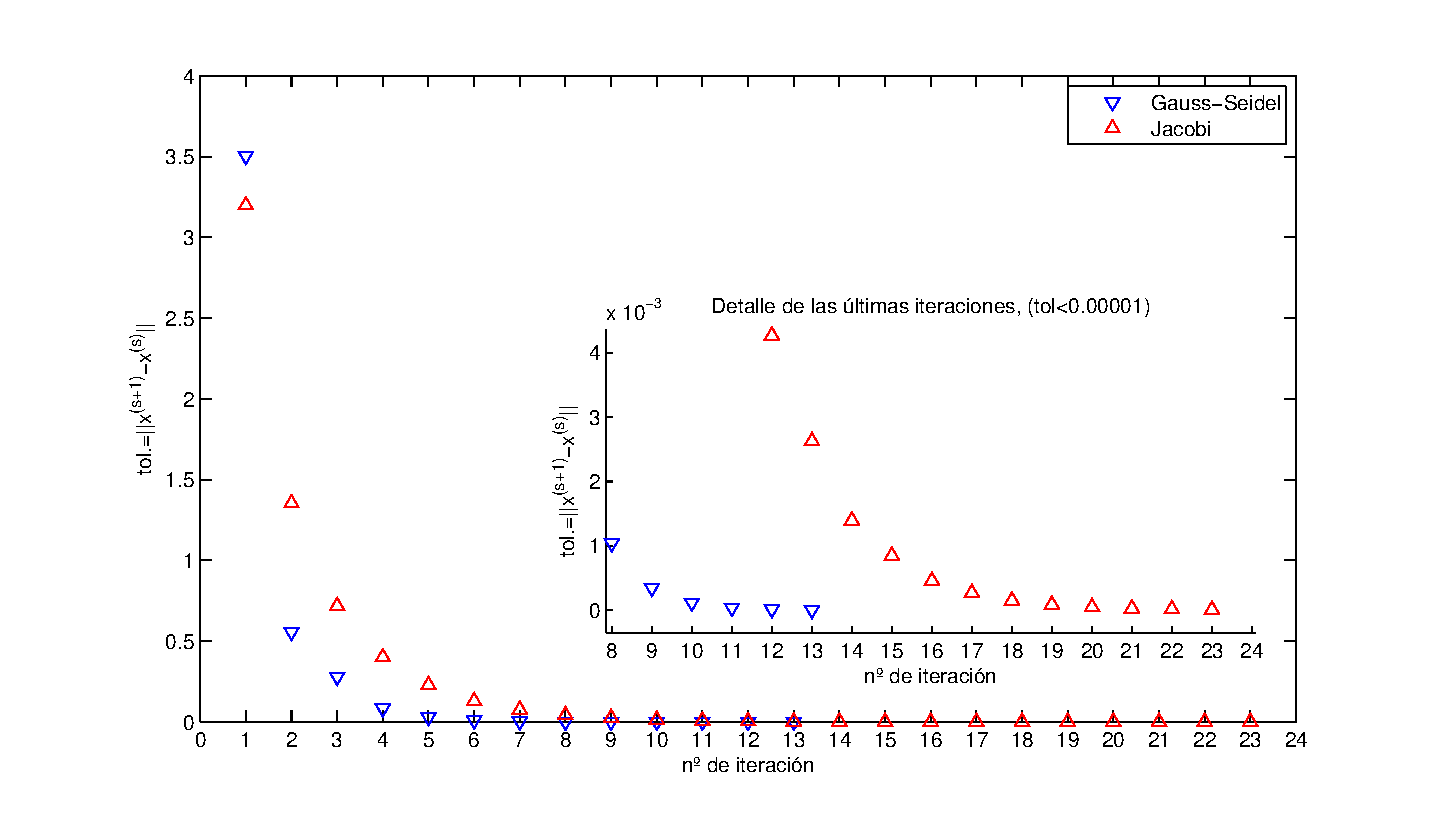
\includegraphics[width=16cm]{gjcom.eps}
\caption{evolución de la tolerancia (módulo de la diferencia entre dos soluciones sucesivas) para un mismo sistema resuelto mediante el método de Gauss-Seidel y el método de Jacobi}
\label{fig:gjcom}
\end{figure}

\subsection{Amortiguamiento.} \index{Métodos amortiguados} El amortiguamiento consiste en modificar un método iterativo, de modo que en cada iteración, se da como solución la media ponderada de los resultados de dos iteraciones sucesivas,
\begin{equation*}
x^{(s+1)}=\omega \cdot x^{*}+(1-\omega) \cdot x^{(s)}
\end{equation*}

Donde $x^{(*)}$ representa el valor que se obtendría aplicando una iteración del método a $x^{(s)}$, es decir sería el valor de $x^{(s+1)}$ si no se aplica amortiguamiento.

El parámetro $\omega$ recibe el nombre de factor de relajamiento. Si $0<\omega<1$ se trata de un método de subrelajación. Su uso permite resolver sistemas que no convergen si se usa el mismo método sin relajación. Si $w>1$ el método se llama de sobrerelajación, permite acelerar la convergencia respecto al mismo método sin relajación. Por último, si hacemos $\omega=1$, recuperamos el método original sin relajación.

\paragraph{El método de Jacobi amortiguado.} \index{Método de Jacobi amortiguado} Se obtiene aplicando el método de relajación que acabamos de describir, al método de Jacobi. La expresión general de una iteración del método de Jacobi amortiguando sería,
\begin{equation*}
x_i^{(s+1)}=\omega\cdot \overbrace{\frac{b_i-\sum_{j\neq i}a_{ij}x_j^{(s)}}{a_{ii}}}^{x^{(*)}}+(1- \omega)\cdot x_i^{s}
\end{equation*}

Para implementarlo en Matlab, bastaría añadir al código del método de Jacobi una línea incluyendo el promedio entre las dos soluciones sucesivas,

\begin{lstlisting}
while norm(xs1-xs)>tol
 	xs=xs1;
    % volvemos a inicializar el vector de soluciones al valor de los
    % terminos independientes
    xs1=b; 
    for i=1:n % bucle para recorrer todas las ecuaciones
        for j=1:i-1 % restamos la contribucion de todas las incognitas
            xs1(i)=xs1(i)-A(i,j)*xs(j);       % por encima de x(i)
        end
        for j=i+1:n % restamos la contribución de todas las incognitas
            % por debajo de x(i)
            xs1(i)=xs1(i)-A(i,j)*xs(j);
        end
        % dividimos por el elemento de la diagonal,
        xs1(i)=xs1(i)/A(i,i);
    end
    % promediamos la solución obtenida con la anterior (amortiguamiento)
    xs1=w*xs1+(1-w)*xs
end
\end{lstlisting}

En forma matricial, la expresión general del método de Jacobi amortiguado sería,

\begin{equation*}
x^{(s+1)}=\omega\cdot\overbrace{\left(D^{-1}\cdot b- D^{-1}\cdot\left(L+U\right)\cdot x^{(s)}\right)}^{x^{(*)}}+(1-w)x^{(s)}
\end{equation*}
Si reorganizamos esta expresión,

\begin{equation*}
x^{(s+1)}=\omega\cdot D^{-1}\cdot b+ \left[(1-w)\cdot I - w\cdot  D^{-1}\cdot  \left(L+U \right)\right]\cdot x^{(s)}
\end{equation*}

Podemos identificar fácilmente el termino fijo, $f=\omega\cdot D^{-1}\cdot b$ y la matriz del método $H=\left((1-w)\cdot I - w\cdot  D^{-1}\cdot  \left(L+U \right)\right)$.

Para implementar el código del método de Jacobi amortiguado en Matlab, debemos calcular la matriz identidad del tamaño de sistema y modificar las expresiones de $f$ y $H$,

\begin{lstlisting}
...
...
% obtenemos el tamaño del sistema,

n=size(A,1);
% creamos un vector de soluciones inicial,
xs=zeros(n,1);
% creamos las matrices del método
D=diag(diag(A));
U=A-tril(A);
L=A-triu(A);
I=eye(n);
% Alternativamente para jacobi podemos crear una solo matriz equivalenta a
% L+U, LpU=A-D
f=w*D^-1*b;
H=-w*D^-1*(L+U)+(1-w)*I;

% calculamos la primera iteración,
xs1=f+H*xs;
% calculamos la diferencia entre las dos soluciones,
tolf=norm(xs1-xs);
% ponemos a 1 el contador de iteraciones.
it=1;

% a partir de aquí vendría el código necesario para calcular las
% sucesivas iteraciones hasta que la solución converja
...
...
\end{lstlisting}

\paragraph{El método SOR.} \index{Método SOR}El método SOR --\emph{Succesive OverRelaxation}-- se obtiene aplicando amortiguamiento al método de Gauss-Seidel. Aplicando el mismo razonamiento que el caso de Jacobi amortiguado, la expresión general para una iteración del método SOR es,

\begin{equation*}
x_i^{(s+1)}=\omega\cdot \overbrace{\frac{b_i-\sum_{j< i}a_{ij}x_j^{(s+1)}-\sum_{j> i}a_{ij}x_j^{(s)}}{a_{ii}}}^{x^{(*)}}+(1-\omega)\cdot x_i^{(s)}
\end{equation*}

Al igual que en el caso de Jacobi amortiguado, para implementar en Matlab el método SOR es suficiente añadir una línea que calcule el promedio de dos soluciones sucesivas,

\begin{lstlisting}
    xs=xs1;
    % volvemos a inicializar el vector de soluciones al valor de los
    % terminos independientes
    xs1=b; 
    for i=1:n % bucle para recorrer todas las ecuaciones
        for j=1:i-1 % restamos la contribucion de todas las incognitas
            xs1(i)=xs1(i)-A(i,j)*xs1(j);       % por encima de x(i)
        end
        for j=i+1:n % restamos la contribución de todas las incognitas
            % por debajo de x(i)
            xs1(i)=xs1(i)-A(i,j)*xs(j);
        end
        % dividimos por el elemento de la diagonal,
        xs1(i)=xs1(i)/A(i,i);
    end
     % amortiguamos la solución
      xs1=w*xs1+(1-w)*xs;
     % calculamos la diferencia entre las dos soluciones,
        tolf=norm(xs1-xs);
        % incrementamos el contador de iteraciones
        it=it+1;
\end{lstlisting}

En forma matricial la expresión para una iteración del método SOR sería,
\begin{equation*}
x^{(s+1)}= \omega\cdot\overbrace{\left((D+L)^{-1}\cdot b-(D+L)^{-1}\cdot U\cdot x^{(s)}\right)}^{x^{(*)}}+(1-\omega)\cdot x^{(s)}
\end{equation*}

Y tras reordenar,

\begin{equation*}
x^{(s+1)}= \omega\cdot\left((D+L)^{-1}\cdot b\right)+\left[(1-\omega)\cdot I-\omega\cdot(D+L)^{-1}\cdot U\right]\cdot x^{(s)}
\end{equation*}

De nuevo, podemos identificar, el término fijo, $f=\omega\cdot\left((D+L)^{-1}\cdot b\right)$ y la matriz del método, $H=\left((1-\omega)\cdot I-\omega\cdot(D+L)^{-1}\cdot U\right)$.

El siguiente fragmento de código muestra la obtención de $f$ y $H$ para el método SOR,

\begin{lstlisting}
% obtenemos el tamaño del sistema,

n=size(A,1);
% creamos un vector de soluciones inicial,
xs=zeros(n,1);
% calculamos las matrices necesarias

D=diag(diag(A));
U=A-tril(A);
L=A-triu(A);
I=eye(n);


f=w*(D+L)^(-1)*b;
H=(1-w)*I-w*(D+L)^(-1)*U;


% calculamos la primera iteración
xs1=f+H*xs;

% calculamos la diferencia entre las dos soluciones,
tolf=norm(x-x0);
% ponemos a 1 el contador de iteraciones.
it=1;
\end{lstlisting}

\subsection{Análisis de convergencia}\index{Análisis de convergencia}
En la introducción a los métodos iterativos dejamos abierta la cuestión de su convergencia. Vamos a analizar en más detalle en qué condiciones podemos asegurar que un método iterativo, aplicado a un sistema de ecuaciones lineales concreto, converge. 

En primer lugar, tenemos que definir qué entendemos por convergencia. Cuando un método iterativo converge, lo hace en forma asintótica. Es decir, haría falta un número infinito de iteraciones para alcanzar la solución exacta.

\begin{equation*}
x^{(0)}\rightarrow x^{(1)} \rightarrow x^{(2)}\rightarrow \cdots \rightarrow x^{(\infty)}=x
\end{equation*}

Lógicamente, es inviable realizar un número infinito de iteraciones. Por esta razón, las soluciones de los métodos iterativos son siempre aproximadas; realizamos un número finito de iteraciones hasta cumplir una determinada condición de convergencia. Como no conocemos la solución exacta, imponemos dicha condición entre dos iteraciones sucesivas,
\begin{equation*}
 \lVert x^{(s+1)}-x^{(s)}\rVert \leq C \Rightarrow  \lVert x^{(s+1)}-x\rVert = \lvert e^{(s+1)} \rvert
\end{equation*}
Donde $e^{(s+1)}$ representaría el error \emph{real} de convergencia cometido en la iteración $s+1$.

Tomando como punto de partida la expresión general del cálculo de una iteración en forma matricial,
\begin{equation*}
x^{(s+1)}=f+H\cdot x^{(s)}
\end{equation*}

Podemos expresar el error de convergencia como,
\begin{equation*}
e^{(s+1)}=x^{(s+1)}-x=f+H\cdot x^{(s)}-x
\end{equation*}

Pero la solución exacta, si pudiera alcanzarse, cumpliría,

\begin{equation*}
x=f+H\cdot x
\end{equation*}

Y si sustituimos en la expresión del error de convergencia,

\begin{equation*}
e^{(s+1)}=f+H\cdot x^{(s)}-f-H\cdot x
\end{equation*}

Llegamos finalmente a la siguiente expresión, que relaciona los errores de convergencia de dos iteraciones sucesivas,

\begin{equation*}
e^{(s+1)}=H\cdot e^{(s)}
\end{equation*}

Para que el error disminuya de iteración en iteración y el método converja, es necesario que la matriz del método $H$ tenga norma-2  menor que la unidad.

Supongamos que un sistema de dimension $n$ su matriz del método $H$, tiene un conjunto de $n$ autovectores linealmente independientes, $w_1, \ w_2, \cdots, \ w_n$, cada uno asociado a su correspondiente autovalor, $\lambda_1, \ \lambda_2, \ \cdots,\ \lambda_n$. El error de convergencia, es también un vector de dimensión $n$, por tanto podemos expresarlo como una combinación lineal de los $n$ autovectores linealmente independientes de la matriz $H$. Supongamos que lo hacemos para el error de convergencia $e^{(0)}$correspondiente al valor inicial de la solución $x^{(0)}$,

\begin{equation*}
e^{(0)}=\alpha_1\cdot w_1+\alpha_2\cdot w_2+\cdots+\alpha_n\cdot w_n
\end{equation*}

Si empleamos la ecuación deducida antes para la relación del error entre dos iteraciones sucesivas y recordando que aplicar una matriz a un autovector, es equivalente a multiplicarlo por el autovalor correspondientes: $H\cdot w_i=\lambda_i\cdot w_i$, obtenemos para el error de convergencia en la iteración $s$,

\begin{align*}
e^{(1)}&=H\cdot e^{(0)}=\alpha_1\cdot \lambda_1 \cdot  w_1+\alpha_2\cdot \lambda_2 \cdot  w_2+\cdots+\alpha_n\cdot \lambda_n \cdot w_n\\
e^{(2)}&=H\cdot e^{(1)}=H^2\cdot e^{(0)}=\alpha_1\cdot \lambda_1^2 \cdot  w_1+\alpha_2\cdot \lambda_2^2 \cdot  w_2+\cdots+\alpha_n\cdot \lambda_n^2 \cdot w_n\\
\vdots \ \ \ & \\
e^{(s)}&=H\cdot e^{(s-1)}=H^s\cdot e^{(0)}=\alpha_1\cdot \lambda_1^s \cdot  w_1+\alpha_2\cdot \lambda_2^s \cdot  w_2+\cdots+\alpha_n\cdot \lambda_n^s \cdot w_n
\end{align*}

Para que el error tienda a cero, $e^{(s)}\rightarrow 0$ al aumentar $s$, para cualquier combinación inicial de valores $\alpha_i$, esto es para cualquier aproximación inicial $x^{(0)}$, es necesario que todos los autovalores de la matriz del método cumplan,

\begin{equation*}
\vert \lambda_i \vert < 1
\end{equation*}

Por tanto, el sistema converge si el radio espectral de la matriz del método es menor que la unidad. \footnote{El radio espectral de una matriz es el mayor de sus autovalores en valor absoluto. Ver capítulo \ref{resp}.}

\begin{equation*}
\rho(H)<1 \Rightarrow \lim_{s\rightarrow \infty}e^{(s)}=0
\end{equation*}

\paragraph{Velocidad de convergencia.} \index{Velocidad de convergencia}Para un número de iteraciones suficientemente grande, el radio espectral de la matriz del método nos da la velocidad de convergencia. Esto es debido a que el resto de los términos del error, asociados a otros autovalores más pequeños tienden a cero más  deprisa. Por tanto podemos hacer la siguiente aproximación, donde estamos suponiendo que el autovalor $\lambda_n$ es el radio espectral,

\begin{equation*}
e^{(s)}\approx c_n \rho(H)^s w_n= c_n \lambda_n^s w_n
\end{equation*}

Podemos ahora calcular cuantas iteraciones nos costará reducir un error inicial por debajo de un determinado valor. Esto dependerá de la solución inicial y de radio espectral de la matriz del método,
\begin{equation*}
e^{(s)}\approx  \rho(H)^s e^{(0)} \Rightarrow \frac{e^{(s)}}{e^{(0)}} \approx \rho(H)^s
\end{equation*}

así por ejemplo si queremos reducir el error inicial en $m$ dígitos,
\begin{equation*}
\frac{e^{(s)}}{e^{(0)}} \approx \rho(h)^s \leq 10^{-m} \Rightarrow s \geq \frac{-m}{\log_{10}\left(\rho(H)\right)}
\end{equation*}

La matriz del método juega por tanto un papel fundamental tanto en la convergencia del método, como en la velocidad (número de iteraciones) con la que el método converge. Los métodos amortiguados, permiten modificar la matriz de convergencia, gracias al factor de amortiguamiento $\omega$, haciendo que sistemas para los que no es posible encontrar una solución mediante un método iterativo converjan.

Como ejemplo, el sistema,

\begin{equation*}
\begin{pmatrix}
1& 2& -1\\
2& -5& 1\\
1& -1& 3
\end{pmatrix}\cdot \begin{pmatrix}
x_1\\
x_2\\
x_3
\end{pmatrix}=\begin{pmatrix}
2\\
-5\\
8
\end{pmatrix}
\end{equation*}

No converge si tratamos de resolverlo por el método de Jacobi. Sin embargo si es posible obtener su solución empleando el método de Jacobi Amortiguado. La figura \ref{fig:cjjam}  muestra la evolución de la tolerancia para dicho sistema empleando ambos métodos.

\begin{figure}[h]
\centering
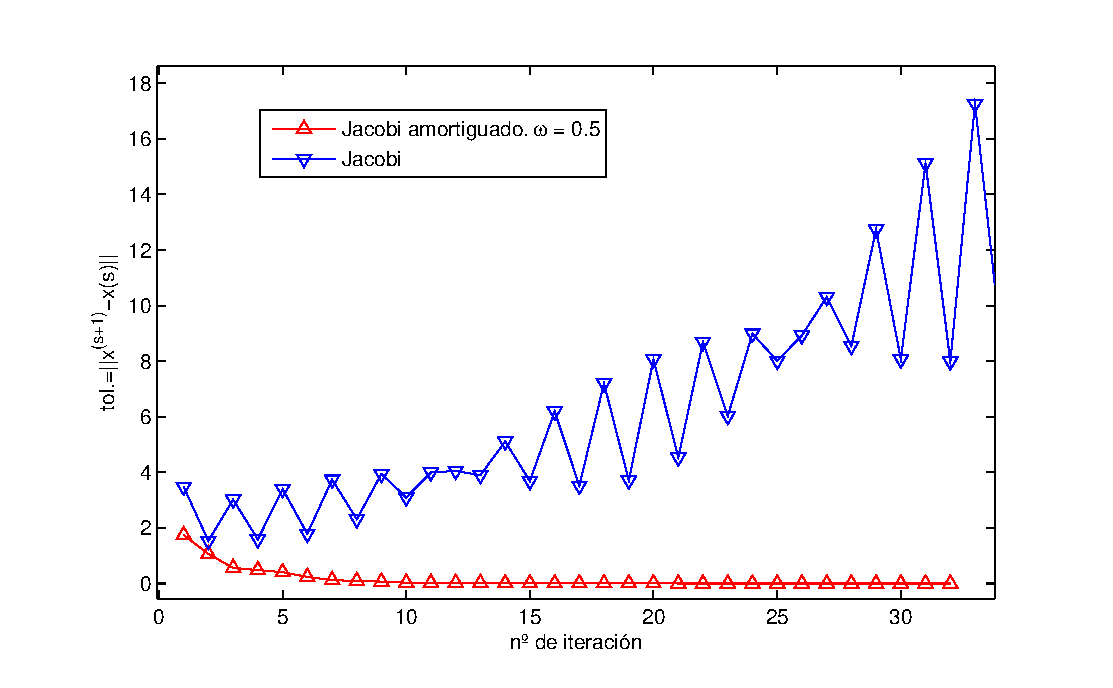
\includegraphics[width=14cm]{comjjam.eps}
\caption{Evolución de la tolerancia para un mismo sistema empleando el metodo de Jacobi (diverge) y el de Jacobi amortiguado (converge).}
\label{fig:cjjam}


\end{figure}

Si calculamos el radio espectral de la matriz del método, para el método de Jacobi tendríamos,
\begin{verbatim}
>> A=[1 2 -1  ; 2 -5 1;1 -1 3]

A =

     1     2    -1
     2    -5     1
     1    -1     3

>> H=diag(diag(A))^-1*(A-diag(diag(A)))

H =

         0    2.0000   -1.0000
   -0.4000         0   -0.2000
    0.3333   -0.3333         0

>> l=eig(H)
l =

   0.1187 + 1.0531i
   0.1187 - 1.0531i
  -0.2374          

>> radio_espectral=max(abs(l))
radio_espectral =

    1.0597
\end{verbatim}

El radio espectral es mayor que la unidad y el método no converge.

Si repetimos el cálculo para el método de Jacobi amortiguado, con $\omega=0.5$
\begin{verbatim}
>> H=(1-0.5)*eye(3)-0.5*diag(diag(A))^-1*(A-diag(diag(A)))

H =

    0.5000   -1.0000    0.5000
    0.2000    0.5000    0.1000
   -0.1667    0.1667    0.5000

>> l=eig(H)

l =

   0.4406 + 0.5265i
   0.4406 - 0.5265i
   0.6187          

>> radio_espectral=max(abs(l))

radio_espectral =

    0.6866
\end{verbatim}

El radio espectral es ahora menor que la unidad y el método converge.

Por último indicar que cualquiera de los métodos iterativos descrito converge para un sistema que cumpla que su matriz de coeficientes es estrictamente diagonal dominante.
\section{Ejercicios}
\begin{enumerate}
\item Crea una función en matlab que calcule la solución de un sistema de ecuaciones triangular inferior empleando el método de sustituciones progresivas. La función deberá tomar como valores de entrada una matriz triangular inferior de dimensión $(n\times n)$ arbitraria y un vector columna $(n\times 1)$ de términos independientes. Deberá devolver como variable de salida un vector columna $(n\times 1)$ con las soluciones del sistema.

\item \label{eje62} Crea una función en matlab que calcule la solución de un sistema de ecuaciones triangular superior empleando el método de sustituciones regresivas. La función deberá tomar como valores de entrada una matriz triangular inferior de dimensión $(n\times n)$ arbitraria y un vector columna $(n\times 1)$ de términos independientes. Deberá devolver un vector columna $(n\times 1)$ con las soluciones del sistema.

\item Crea una función que dadas una matriz cuadrada  $ A,\ (n\times n)$ y un  vector columna $b,\ (n\times 1)$, construya la matriz ampliada $Ab$, Aplique el método de eliminación gausiana a la matriz ampliada y llame a la función creada en el ejercicio \ref{eje62} Para resolver el sistema $Ax=b$. La función deberá devolver como variables de salida, La matriz resultante de la aplicar la eliminación gaussiana a la ampliada y un vector columna con las soluciones del sistema resuelto. 

\item Crea una función que dadas una matriz cuadrada  $ A,\ (n\times n)$ y un  vector columna $b,\ (n\times 1)$, construya la matriz ampliada $Ab$,aAplique el método de eliminación Gauss-Jordan a la matriz ampliada y devuelva como variable de salida la matriz en forma escalonada reducida por filas, de modo que la última fila sea la solución del sistema $Ax=b$  

\item Construye un programa que resuelva un sistema de ecuaciones de dimensión arbitraria, empleando el método de Jacobi simple (no en forma matricial). El programa deberá admitir como variables de entrada, una matriz de coeficientes $ A,\ (n\times n)$, un vector de términos independientes $b,\ (n\times 1)$, una solución inicial $x_0 ,\ (n\times 1)$, un valor para la tolerancia máxima entre dos iteraciones sucesivas y un número máximo de iteraciones permitido. El programa deberá devolver un vector columna con las soluciones del sistema, el número de iteraciones empleado y el error relativo entre las dos últimas iteraciones realizadas.

\item Repite el ejercicio anterior empleando ahora el método de Jacobi matricial. Añade el código necesario para que calcule en primer lugar el radio espectral de la matriz del método y caso de no cumplirse  la condición de convergencia, el programa interrumpa su ejecución y devuelva un mensaje de error indicando el valor del radio espectral.

\item Construye un programa que resuelva un sistema de ecuaciones de dimensión arbitraria, empleando el método de Gauss-Seidel simple (no en forma matricial). El programa deberá admitir como variables de entrada, una matriz de coeficientes $ A,\ (n\times n)$, un vector de términos independientes $b,\ (n\times 1)$, una solución inicial $x_0 ,\ (n\times 1)$, un valor para la tolerancia máxima entre dos iteraciones sucesivas y un número máximo de iteraciones permitido. El programa deberá devolver un vector columna con las soluciones del sistema, el número de iteraciones empleado y el error relativo entre las dos últimas iteraciones realizadas.

\item Repite el ejercicio anterior empleando ahora el método de Gauss-Seidel matricial. Añade el código necesario para que calcule en primer lugar el radio espectral de la matriz del método y caso de no cumplirse  la condición de convergencia, el programa interrumpa su ejecución y devuelva un mensaje de error indicando el valor del radio espectral.

\item Construye un programa que resuelva un sistema de ecuaciones de dimensión arbitraria, empleando el método de Jacobi amortiguado simple (no en forma matricial). El programa deberá admitir como variables de entrada, una matriz de coeficientes $ A,\ (n\times n)$, un vector de términos independientes $b,\ (n\times 1)$, una solución inicial $x_0 ,\ (n\times 1)$, un valor para el parámetro de amortiguamiento $\omega$, un valor para la tolerancia máxima entre dos iteraciones sucesivas y un número máximo de iteraciones permitido. El programa deberá devolver un vector columna con las soluciones del sistema, el número de iteraciones empleado y el error relativo entre las dos últimas iteraciones realizadas.

\item Repite el ejercicio anterior empleando ahora el método de Jacobi amortiguado matricial. Añade el código necesario para que calcule en primer lugar el radio espectral de la matriz del método y caso de no cumplirse  la condición de convergencia, el programa interrumpa su ejecución y devuelva un mensaje de error indicando el valor del radio espectral.

\item Construye un programa que resuelva un sistema de ecuaciones de dimensión arbitraria, empleando el método SOR  simple (no en forma matricial). El programa deberá admitir como variables de entrada, una matriz de coeficientes $ A,\ (n\times n)$, un vector de términos independientes $b,\ (n\times 1)$, una solución inicial $x_0 ,\ (n\times 1)$, un valor para el parámetro de amortiguamiento $\omega$, un valor para la tolerancia máxima entre dos iteraciones sucesivas y un número máximo de iteraciones permitido. El programa deberá devolver un vector columna con las soluciones del sistema, el número de iteraciones empleado y el error relativo entre las dos últimas iteraciones realizadas.

\item Repite el ejercicio anterior empleando ahora el método SOR matricial. Añade el código necesario para que calcule en primer lugar el radio espectral de la matriz del método y caso de no cumplirse  la condición de convergencia, el programa interrumpa su ejecución y devuelva un mensaje de error indicando el valor del radio espectral.


\item Resuelve el siguiente sistema de ecuaciones, empleando las factorización LU de matlab. Indica todos los pasos empleados hasta obtener las solución del sistema. \textbf{(1.5 puntos)}
\begin{align*}
3x_1&+3x_2-2x_3 +\ x_4= 13\\
 &+2x_2-\ x_3  \hspace{30pt} =\ 3\\
-2x_1&+\ x_2 + 5x_3 -4x_4=\ 1\\
2x_1& \hspace{30pt} -\ x_3 +2x_4 =\ 5
\end{align*}
Repite el ejercicio empleando las factorizaciones QR y SVD.

\item Para calcular las intensidades de un circuito de corriente continua como el de la figura, es suficiente emplear las leyes de Kirchoff. La primera ley --\emph{ley de nodos}-- establece que la suma de corrientes que llegan a un nodo del circuito debe ser igual a cero.
La segunda --\emph{ley de mallas}-- establece que la suma de las caídas de tensión en un malla cerrada tiene que ser cero. La caída de voltaje en una resistencia se calcula empleando la ley de Ohm: $V = i\cdot R$
Si aplicamos las leyes de Kirchoff al circuito de la figura, obtenemos  el siguiente sistema de ecuaciones,

\begin{minipage}{0.3\textwidth}
\begin{align*}
i_1 - i_2 - i_3 &= 0\\
i_3 - i_4 - i_5 &= 0\\
i_5  + i_2 -i_6&= 0\\
5i_3 + 70 i_4 &= 180\\
25i_2 -5i_3-10i_5 &= 0\\
10i_5+8i_6 -70i_4 &= 0  
\end{align*}
\end{minipage}
\begin{minipage}{0.7\textwidth}
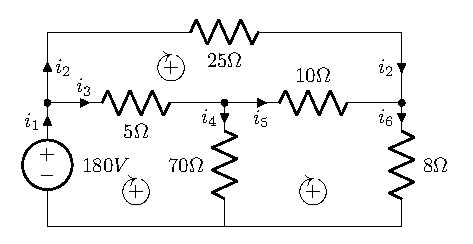
\includegraphics[scale=1.1]{circuito.eps}
\end{minipage}
\ \\
Las tres primeras ecuaciones corresponden a aplicar la \emph{ley de nodos} a los nodos marcados con un punto negro en la figura. 

Las tres últimas, a aplicar la \emph{ley de mallas} a las tres mallas considerando positivo recorrerlas en el sentido de las agujas del reloj.

El sistema de ecuaciones obtenido puede expresarse en forma matricial como,
\begin{equation}\label{cucu}
\begin{pmatrix}
1& -1& -1& 0 & 0 &0\\
0& 0& 1& -1& -1& 0\\
0& 1& 0&  0&  1& -1\\ 
0& 0& 5& 70& 0& 0\\
0& 25& -5& 0& -10& 0\\
0& 0& 0& -70& 10& 8
\end{pmatrix}\begin{pmatrix}
i_1\\ i_2\\ i_3\\ i_4\\ i_5\\ i_6
\end{pmatrix}= \begin{pmatrix}
0\\ 0\\ 0\\ 180\\ 0\\ 0
\end{pmatrix} 
\end{equation}



\begin{enumerate}
\item Define en Matlab{$^\copyright$} el sistema de ecuaciones (\ref{cucu}). Obtén los valores de las intensidades en todas las ramas del circuito empleando directamente un solo comando o función de Matlab{$^\copyright$}. Emplea el comando \texttt{cond} y dí si en tu opinión el sistema está bien o mal condicionado. (1 punto)

\item Emplea la factorización QR para obtener de nuevo la solución del sistema.  (1 punto)

\item Utilizando la versión permutada del sistema, obtenida mediante la factorización LU, es decir, usando $P\cdot A$ como matriz del sistema y $P\cdot b$, como término independiente, calcula el radio espectral correspondiente al método de Jacobi e indica si tiene sentido o no emplear este método para obtener las intensidades del circuito de la figura. (2 puntos)

\item Emplea el método de Jacobi amortiguado, con un amortiguamiento de $\omega =0.1$ para calcular las intensidades del circuito de la figura, con una tolerancia de $10^{-5}$. Indica el número de iteraciones empleado hasta alcanzar la solución.  (\emph{Nota importante:} Usa la versión permutada del sistema y ten en cuenta que va a necesitar bastantes iteraciones --más de $3000$-- para converger). (2 puntos)

\item Emplea el método SOR, con un amortiguamiento de $\omega =0.2$ para calcular las intensidades del circuito de la figura, con una tolerancia de $10^{-5}$. Indica el número de iteraciones empleado hasta alcanzar la solución (\emph{Nota importante:} Usa la versión permutada del sistema).
Discute, a la vista de los resultados, cúal método funciona mejor. (2 puntos)

\item Escribe un código que permita dibujar el radio espectral de un método amortiguado en función de la matriz del método, para distintos valores del amortiguamiento. Emplea el programa para los casos de las dos preguntas anteriores. ¿Ha sido razonable la elección de los valores de $\omega$ realizada en dichas preguntas? (2 puntos) 
\end{enumerate}
\end{enumerate}

\section{Test del curso 2020/21}
\noindent \textbf{Problema 1}. El método iterativo de Richardson para la resolución de sistemas de ecuaciones lineales emplea la siguiente fórmula de recurrencia
\begin{equation}\label{eq:1}
x^{(s+1)} = x^{(s)} + \omega\left( b - Ax^{(s)}\right),
\end{equation}  
		donde $A \in \mathbb{R}^{n\times n}$ y $b  \in \mathbb{R}^{n}$ representan respectivamente la matriz de coeficientes y el vector columna de términos independientes del sistema de ecuaciones $Ax=b$ de orden $n\in\mathbb{N}$, y $x^{(s)}\in\mathbb{R}^n$ es el vector solución en la iteración $s\in\mathbb{N}$. El parámetro $\omega \in \mathbb{R}$  juega el mismo papel que el factor de relajación en los métodos amortiguados y debe ajustarse para asegurar la convergencia del método.

 \begin{enumerate}
\item {\bf 1 punto.} Reescribe la fórmula de recurrencia del método Richardson (ecuación \ref{eq:1})  en la forma matricial estándar
\begin{equation}\label{eq:2}
x^{(s+1)} = f + Hx^{(s)}.
\end{equation}

\item {\bf 2 puntos.} Construye una función em Matlab que implemente el método de Richardson enpleando la forma matricial estándar, es decir, en cada iteración aplicamos la ecuación (\ref{eq:2}). La función deberá tomar como variables de entrada: 
\begin{enumerate}
	\item La matriz de coeficientes $A$.
	\item El vector de términos independientes $b$.
	\item El valor inicial $x^{(0)}$.
	\item Número máximo de iteraciones a realizar.
	\item Tolerancia mínima para el error entre iteraciones sucesivas.
	\item Un valor para el parámetro $\omega$.
\end{enumerate}
Así mismo, la función deberá devolver como variables de salida: 
\begin{enumerate}
\item La solución del sistema.
\item La tolerancia alcanzada.
\item El número de iteraciones empleado en obtener la solución.
\end{enumerate}

\item {\bf 2 puntos.} Emplea los métodos de Richardson, Jacobi y Gauss-Seidel para obtener la solución del sistema de ecuaciones
\begin{equation*}
\begin{pmatrix}
5&2&3&-1\\
2&6&3&0\\
1&-4&4&-1\\
2&0&3&7
\end{pmatrix}\begin{pmatrix}
x_1\\ x_2\\ x_3\\ x_4
\end{pmatrix}= \begin{pmatrix}
14\\ 23\\1\\ 39
\end{pmatrix}.
\end{equation*}
		 Emplea un valor $\omega = 0.16$ para el método de Richardson y una tolerancia de $10^{-5}$ para los tres métodos. Escoge el valor $x^{(0)}=\left[0,0,0,0\right]^T$ para los tres métodos.

Clasifica los tres métodos de mejor a peor, tomando como criterio el número de iteraciones empleado por cada uno de ellos para alcanzar la solución.

% \item {\bf 2 puntos.} \textcolor{red}{Define el error de la solución propuesta en la iteración $s$ con respecto al valor real de la solución $x$, esto es, $e^{(s)} = x^{(s)} - x$. Halla la matriz $W\in\mathbb{R}^{n\times n}$ que satisface:}
%	\begin{equation}
%		e^{(s+1)} = We^{(s)}.
%		\label{eq: error}
%	\end{equation}
%	 Metodología/pista: Sustituye $x^{(s)} = e^{(s)} + x$ en (\ref{eq:1}), y opera hasta alcanzar (\ref{eq: error}).

\item {\bf 2 punto.} Haz una gráfica del radio espectral de $H$ en función del parámetro $\omega$ para el método de Richardson y el sistema de ecuaciones del apartado anterior. Emplea para ello valores de $\omega$ comprendidos en el intervalo $[0.01\ 0.9]$, toma una separación entre valores de $0.01$.  Representa cada valor como un punto independiente.

Determina, a la vista de la gráfica, si sería posible encontrar un valor de $\omega$ para el que se alcance la solución del sistema en menos iteraciones, manteniendo la misma tolerancia. Indica, también de acuerdo con el gráfico, cuál es mayor valor de $\omega$ admisible. Razona las respuestas.
\end{enumerate}

\noindent \textbf{Problema 2.} El método de Gauss-Jordan permite resolver sistemas de ecuaciones lineales de la forma $Ax =b, A \in \mathbb{R}^{n\times n}$ y $x,b  \in \mathbb{R}^{n}$. Si en lugar de emplear un vector columna de términos independientes, sustituimos $b$ por una matriz $B$ de dimensión $n\times m$, el método nos permite obtener como resultado una matriz de soluciones $X$ también de dimension  $n\times m$: $AX=B$. Cada columna, $x_j, \, j\in\{1,\dots,m\}$, de la matriz $X$ representa la solución de sistema $Ax_j=b_j$, donde $b_j$ es la columna correspondiente de la matriz $B$. Es decir: hemos resuelto $m$ sistemas de ecuaciones simultáneamente.

\begin{enumerate}
\item {\bf 2 puntos.} Emplea el método de Gauss-Jordan para obtener la solución de $AX=B$, donde $A$ es la matriz de coeficientes del Problema 1 y B es la matriz identidad de dimension $4\times4$.
\item {\bf 1 punto.} ¿Sabrías decir que relación hay entre las matrices X y A?
\end{enumerate}



